%%%%%%%%%%%%%%%%%%%%%%%%%%%%%%%%%%%%%%%%%%%%%%%%%%%%%%%%%%%%%%%%%%%%%
%% This is a (brief) model paper using the achemso class
%% The document class accepts keyval options, which should include
%% the target journal and optionally the manuscript type.
%%%%%%%%%%%%%%%%%%%%%%%%%%%%%%%%%%%%%%%%%%%%%%%%%%%%%%%%%%%%%%%%%%%%%
\documentclass[journal=jacsat,manuscript=article]{achemso}
\usepackage{subcaption}
\usepackage{amsmath}
\usepackage{amssymb}
\usepackage{graphicx}
\usepackage{array}
\usepackage{adjustbox}
\usepackage{longtable}
\usepackage{xcolor}
\usepackage[normalem]{ulem}
%\usepackage[version=3]{mhchem} % Formula subscripts using \ce{}

%%%%%%%%%%%%%%%%%%%%%%%%%%%%%%%%%%%%%%%%%%%%%%%%%%%%%%%%%%%%%%%%%%%%%
%% If issues arise when submitting your manuscript, you may want to
%% un-comment the next line.  This provides information on the
%% version of every file you have used.
%%%%%%%%%%%%%%%%%%%%%%%%%%%%%%%%%%%%%%%%%%%%%%%%%%%%%%%%%%%%%%%%%%%%%
%%\listfiles

%%%%%%%%%%%%%%%%%%%%%%%%%%%%%%%%%%%%%%%%%%%%%%%%%%%%%%%%%%%%%%%%%%%%%
%% Place any additional macros here.  Please use \newcommand* where
%% possible, and avoid layout-changing macros (which are not used
%% when typesetting).
%%%%%%%%%%%%%%%%%%%%%%%%%%%%%%%%%%%%%%%%%%%%%%%%%%%%%%%%%%%%%%%%%%%%%
\newcommand*\mycommand[1]{\texttt{\emph{#1}}}
\definecolor{revcolor}{RGB}{0,51,153}

%%%%%%%%%%%%%%%%%%%%%%%%%%%%%%%%%%%%%%%%%%%%%%%%%%%%%%%%%%%%%%%%%%%%%
%% Meta-data block
%% ---------------
%% Each author should be given as a separate \author command.
%%
%% Corresponding authors should have an e-mail given after the author
%% name as an \email command. Phone and fax numbers can be given
%% using \phone and \fax, respectively; this information is optional.
%%
%% The affiliation of authors is given after the authors; each
%% \affiliation command applies to all preceding authors not already
%% assigned an affiliation.
%%
%% The affiliation takes an option argument for the short name.  This
%% will typically be something like "University of Somewhere".
%%
%% The \altaffiliation macro should be used for new address, etc.
%% On the other hand, \alsoaffiliation is used on a per author basis
%% when authors are associated with multiple institutions.
%%%%%%%%%%%%%%%%%%%%%%%%%%%%%%%%%%%%%%%%%%%%%%%%%%%%%%%%%%%%%%%%%%%%%
\author{Juan Gomez Quispe}
\affiliation[Universidade Federal do ABC]
{Center of Natural and Human Sciences, Federal University of ABC, Santo André, São Paulo, Brazil}

\author{Caique Campos de Oliveira}
\affiliation[Universidade Federal do ABC]
{Center of Natural and Human Sciences, Federal University of ABC, Santo André, São Paulo, Brazil}

\author{Carlos Raul Primo Sapillado}
\affiliation[National University of San Marcos]
{Facultad de Ciencias Físicas, Universidad Nacional Mayor de San Marcos, 15081 Lima, Perú}

\author{C Rojas-Ayala}
\affiliation[National University of San Marcos]
{Facultad de Ciencias Físicas, Universidad Nacional Mayor de San Marcos, 15081 Lima, Perú}

\author{Pedro Alves Da Silva Autreto}
\affiliation[Universidade Federal do ABC]
{Center of Natural and Human Sciences, Federal University of ABC, Santo André, São Paulo, Brazil}

\email{pedro.autreto@ufabc.edu.br}
\phone{+55 (19) 98279-4988}

%%%%%%%%%%%%%%%%%%%%%%%%%%%%%%%%%%%%%%%%%%%%%%%%%%%%%%%%%%%%%%%%%%%%%
%% The document title should be given as usual. Some journals require
%% a running title from the author: this should be supplied as an
%% optional argument to \title.
%%%%%%%%%%%%%%%%%%%%%%%%%%%%%%%%%%%%%%%%%%%%%%%%%%%%%%%%%%%%%%%%%%%%%
\title[An \textsf{achemso} demo]
{
  Coordination-Dependent Hydrogen Adsorption on Co-, Fe-, and Ni-Functionalized Monolayer CrCl$_{3}$
}

%%%%%%%%%%%%%%%%%%%%%%%%%%%%%%%%%%%%%%%%%%%%%%%%%%%%%%%%%%%%%%%%%%%%%
%% Some journals require a list of abbreviations or keywords to be
%% supplied. These should be set up here, and will be printed after
%% the title and author information, if needed.
%%%%%%%%%%%%%%%%%%%%%%%%%%%%%%%%%%%%%%%%%%%%%%%%%%%%%%%%%%%%%%%%%%%%%
\setkeys{acs}{keywords = true}
\abbreviations{2d-CrCl$_{3}$, TMF, HA, magnetic-2d}
\keywords{Monolayer-CrCl$_{3}$, Transition-metal functionalization, Hydrogen Adsorption, Magnetic two-dimensional materials}

%%%%%%%%%%%%%%%%%%%%%%%%%%%%%%%%%%%%%%%%%%%%%%%%%%%%%%%%%%%%%%%%%%%%%
%% The manuscript does not need to include \maketitle, which is
%% executed automatically.
%%%%%%%%%%%%%%%%%%%%%%%%%%%%%%%%%%%%%%%%%%%%%%%%%%%%%%%%%%%%%%%%%%%%%
\begin{document}

%%%%%%%%%%%%%%%%%%%%%%%%%%%%%%%%%%%%%%%%%%%%%%%%%%%%%%%%%%%%%%%%%%%%%
%% The "tocentry" environment can be used to create an entry for the
%% graphical table of contents. It is given here as some journals
%% require that it is printed as part of the abstract page. It will
%% be automatically moved as appropriate.
%%%%%%%%%%%%%%%%%%%%%%%%%%%%%%%%%%%%%%%%%%%%%%%%%%%%%%%%%%%%%%%%%%%%%
\begin{tocentry}
  \centering
  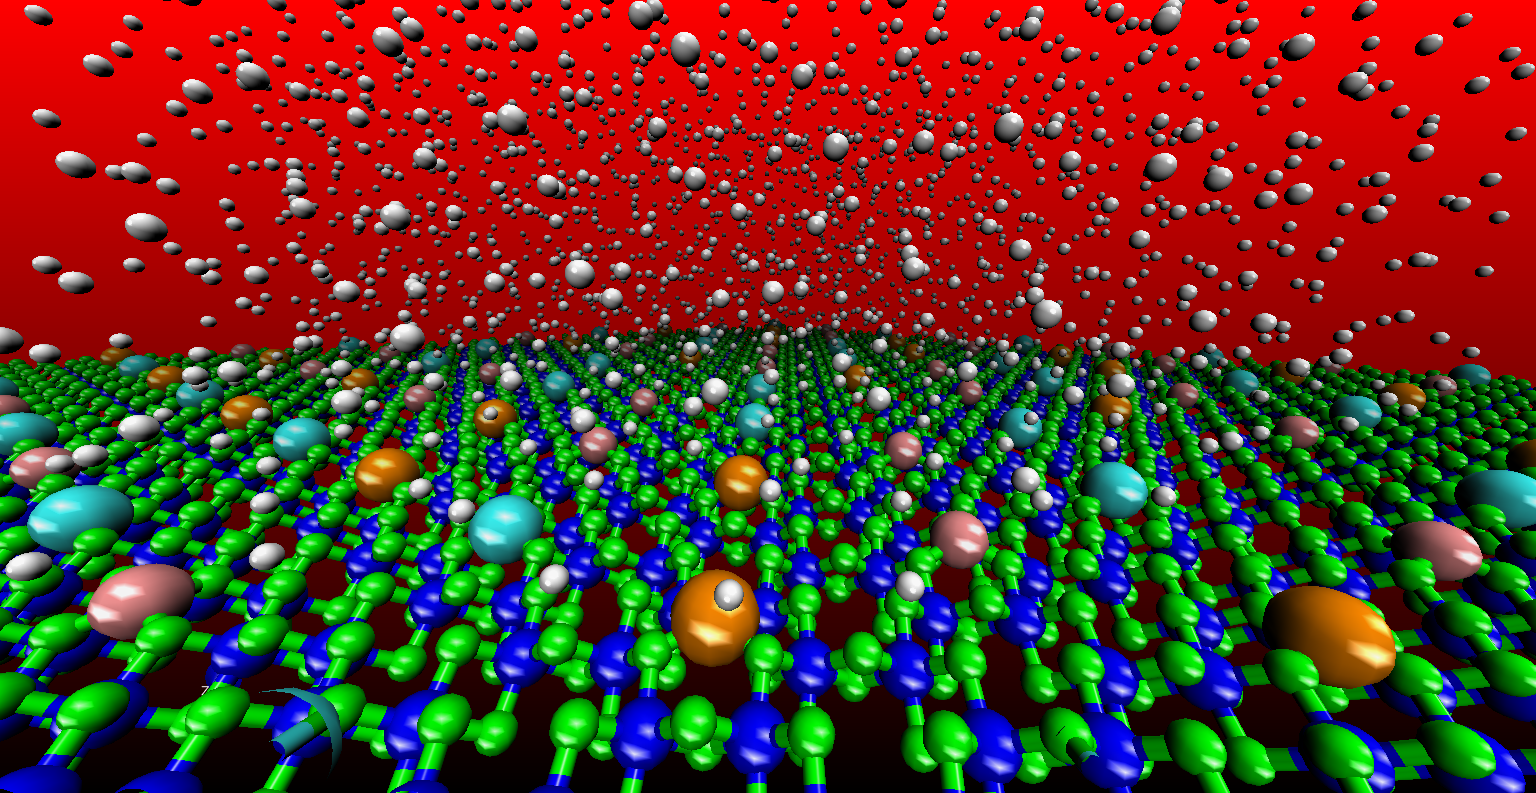
\includegraphics[scale=0.625]{figure/toc.png}
\end{tocentry}

%%%%%%%%%%%%%%%%%%%%%%%%%%%%%%%%%%%%%%%%%%%%%%%%%%%%%%%%%%%%%%%%%%%%%
%% The abstract environment will automatically gobble the contents
%% if an abstract is not used by the target journal.
%%%%%%%%%%%%%%%%%%%%%%%%%%%%%%%%%%%%%%%%%%%%%%%%%%%%%%%%%%%%%%%%%%%%%

\begin{abstract}

  Developing cost-effective two-dimensional (2D) magnetic catalysts for the hydrogen evolution reaction (HER) requires precise control over spin polarization, active-site exposure, and local chemical environments. Here, using spin-polarized density functional theory and ab initio molecular dynamics simulations, we investigate how transition-metal ($\text{TM} = \text{Co}$, $\text{Fe}$, $\text{Ni}$) functionalization and site coordination govern hydrogen adsorption on monolayer $\text{CrCl}_3$. While pristine $\text{CrCl}_3$ exhibits highly unfavorable H-adsorption thermodynamics ($\Delta G_{\text{ads}} = 1.82~\text{eV}$), surface-adsorbed metals introduce localized, spin-polarized $3d$ states that drastically enhance HER propensity. We identify a coordination-controlled trade-off: strong substrate binding does not guarantee optimal catalytic activity. Although Ni binds most strongly to the $\text{CrCl}_3$ lattice and tends toward deeper incorporation at 300~K, surface-adsorbed Co achieves the most favorable, near-thermoneutral adsorption free energy ($\Delta G_{\text{ads}} = 0.20~\text{eV}$, compared to 0.51 and 0.88~\text{eV} for Fe and Ni, respectively). Transitioning from threefold surface sites to sixfold embedded configurations systematically suppresses H binding ($\Delta G_{\text{ads}}$ reaching up to 3.62~\text{eV} for embedded Ni), as increased TM--Cl coordination reduces the orbital accessibility of the metal center and incurs severe geometric deformation penalties. COHP analyses and energy decomposition demonstrate that surface-exposed sites optimize the balance between catalyst stability and active-site reactivity. These findings establish coordination engineering as a key paradigm for tuning catalytic activity in 2D magnetic materials .
\end{abstract}

%%%%%%%%%%%%%%%%%%%%%%%%%%%%%%%%%%%%%%%%%%%%%%%%%%%%%%%%%%%%%%%%%%%%%
%% Start the main part of the manuscript here.
%%%%%%%%%%%%%%%%%%%%%%%%%%%%%%%%%%%%%%%%%%%%%%%%%%%%%%%%%%%%%%%%%%%%%

\section{Introduction}

\noindent Green hydrogen (H$_2$), produced through water electrolysis, holds considerable potential for the decarbonization of hard-to-abate sectors owing to its versatility in clean and renewable energy conversion and storage \cite{ZAINAL2024113941, SAKTHIMURUGAN2025104849}. Beyond its relevance to the energy transition, H$_2$ is also in high demand across several industrial sectors, including fertilizer and steel production and transportation \cite{pr12020315, ROPER2025687}. However, the large-scale implementation of H$_2$-based technologies remains limited by several factors \cite{SAKTHIMURUGAN2025104849, Odenweller2025}, including the need for efficient, stable, and low-cost electrocatalysts for the hydrogen evolution reaction (HER) \cite{Liao2022,Ipaves2025,doi:10.1021/acsaem.6c00060,doi:10.1021/acsomega.5c07529,quispe2026controllingactivitystabilitygamma}. In this context, two-dimensional (2D) materials have attracted considerable attention because their reduced dimensionality, high surface-to-volume ratio, and chemically accessible active sites provide favorable characteristics for catalytic applications \cite{doi:10.1021/acsaem.6c00060, DEYACSAPPENERMATER2026}.

Beyond conventional nonmagnetic 2D systems, intrinsic 2D magnetic materials introduce an additional degree of freedom for catalyst design, since their spin-polarized electronic structures can influence charge transfer, orbital hybridization, adsorption energetics, and surface reactivity \cite{Ipaves2025,doi:10.1021/acscatal.2c06319,Sun2023,Duan2021}. Among these materials, chromium trihalides, CrX$_3$ (X = Cl, Br, I), constitute a particularly versatile family owing to the interplay between their electronic structure, magnetic ordering, anisotropy, and response to external perturbations \cite{Soriano2020,Besbes2019,Lee2026,Kvashnin2020,GarridoAldea2025}.

Within this family, monolayer CrCl$_3$ is an appealing platform for investigating chemically functionalized magnetic catalysts. It is a 2D magnetic semiconductor whose electronic structure and magnetic response can be strongly modified by strain, defects, adsorption, chemical functionalization, and interfacial perturbations \cite{Xue2019,Webster2018,Dupont2021,Zhu2025}. CrCl$_3$ is also experimentally accessible. Bulk crystals have been synthesized by chemical vapor transport and self-transport methods \cite{Abdel-Hafiez2025,Mastrippolito2021}, while atomically thin layers can be isolated through mechanical exfoliation \cite{Kazim_2020}. Exfoliated CrCl$_3$ exhibits comparatively good environmental stability relative to more reactive chromium trihalides such as CrI$_3$ \cite{Mastrippolito2021}. In addition, epitaxial and vapor-phase growth routes have enabled the fabrication of CrCl$_3$ layers down to the monolayer limit \cite{Bedoya2021,Wang2022}. These advances establish CrCl$_3$ as a realistic host material for exploring chemically modified 2D magnetic systems.

The weak magnetic anisotropy of CrCl$_3$ compared with heavier chromium trihalides makes its magnetic state particularly responsive to external stimuli, including strain, electric fields, adsorption, and chemical modification \cite{Webster2018,Ebrahimian2023,Esteras2023}. Its low-dimensional magnetic behavior has consequently motivated extensive investigations of exchange interactions, magnetic excitations, spin textures, and defect-induced phenomena \cite{Sarkar2021,Stagraczynski2024,Esquembre-Kucukalic2025,Lu2020,Mastrippolito2021}. Experimental and theoretical studies have further demonstrated that foreign species, vacancies, and substitutional dopants can substantially modify the electronic structure, magnetic ordering, and local bonding environment of CrCl$_3$ \cite{Luo2020,Gao2018,Mastrippolito2021,Mastrippolito2022}. Related investigations involving Ni incorporation, Fe-doped CrCl$_3$ under pressure, and other transition-metal modifications also indicate that the CrCl$_3$ lattice can accommodate significant chemical and structural perturbations \cite{Wang2019,Abdel-Hafiez2025,Safi2023}.

From a catalytic perspective, the hydrogen adsorption properties of pristine CrCl$_3$ have received considerably less attention than its magnetic properties. Previous first-principles calculations have examined its possible application in HER-related processes \cite{Zala2024}; however, a systematic analysis connecting adsorption-site stability, local coordination, electronic reconstruction, and H-binding thermodynamics remains limited. In particular, the chemically saturated surface of pristine CrCl$_3$ may restrict the formation of accessible adsorption centers. Transition-metal functionalization therefore represents a promising strategy for introducing exposed and electronically active sites while retaining the structural and magnetic characteristics of the 2D host.

Among the $3d$ transition metals, Co, Fe, and Ni are suitable candidates for this purpose because their partially occupied $d$ orbitals can hybridize with the Cr--Cl framework, redistribute charge near the Fermi level, and generate distinct local magnetic and chemical environments. Co, Fe, and Ni carry $d^7$, $d^6$, and $d^8$ electron configurations, respectively, placing them near the thermoneutral region of the HER volcano plot where $\Delta G_{\mathrm{ads}}$ can be tuned toward zero by controlling the local coordination environment \cite{Norskov_2005,Moraes2026}. Earlier $3d$ metals (e.g., Ti, V) tend to overbind H, while late metals with filled $d$-shells (e.g., Cu, Zn) offer limited hybridization. Co, Fe, and Ni also carry significant magnetic moments ($1$--$4~\mu_{\mathrm{B}}$) compatible with the Cr$^{3+}$ ($d^3$) Heisenberg ferromagnet ground state of CrCl$_3$, enabling spin--coordination--catalysis coupling. They are furthermore among the most commonly reported TM functionalization agents for CrCl$_3$ and related chromium trihalides in both theoretical~\cite{Luo2020,Gao2018} and experimental studies~\cite{Mastrippolito2021,Abdel-Hafiez2025}, establishing their experimental realizability. Importantly, their hydrogen adsorption response is expected to depend not only on the chemical identity of the metal but also on its coordination within the CrCl$_3$ lattice. A surface-adsorbed atom may remain accessible for direct interaction with hydrogen, whereas deeper incorporation into the hollow region may increase metal--substrate bonding while reducing the chemical accessibility of the metal center. Despite the extensive literature on strain, defects, adsorption, and selected dopants in CrCl$_3$, a systematic comparison of Co-, Fe-, and Ni-functionalized monolayers in both surface-adsorbed and embedded configurations, specifically in the context of hydrogen adsorption, remains lacking.

In this work, spin-polarized density functional theory (DFT) calculations are employed to investigate Co, Fe, and Ni functionalization of monolayer CrCl$_3$ at the hollow site, considering both adsorbed and embedded motifs. Their relative stability and finite-temperature behavior are evaluated through structural optimization and \textit{ab initio} molecular dynamics simulations. Electronic-structure, charge-transfer, magnetic, and chemical-bonding analyses are then used to determine how metal coordination modifies the CrCl$_3$ host and its interaction with hydrogen. The hydrogen adsorption free energy, $\Delta G_{\mathrm{ads}}$, is employed as a thermodynamic descriptor of HER propensity at the sites and coverage considered here. The results show that pristine CrCl$_3$ exhibits unfavorable H-binding thermodynamics within the investigated configurations, whereas transition-metal functionalization modifies the H-binding thermodynamics in a highly selective manner. Although Ni interacts most strongly with the substrate, surface-adsorbed Co provides the most favorable H adsorption free energy. In contrast, the higher coordination of the embedded metal centers leads to substantially less favorable H adsorption. These findings demonstrate that the hydrogen adsorption response of functionalized CrCl$_3$ is governed by the balance between active-site exposure, local coordination, electronic reconstruction, metal--substrate bonding, and H-binding thermodynamics, rather than by the dopant anchoring strength alone.

\section{Computational Methods}

\noindent All calculations were performed on the (001) basal plane of monolayer CrCl$_3$, i.e., the Cl-terminated surface exposed upon mechanical exfoliation or vapor-phase growth. This is the only chemically accessible surface for a free-standing 2D monolayer and is consistent with the CrCl$_3$ literature~\cite{Webster2018,Mastrippolito2021,Zala2024}. The present study targets the hydrogen evolution reaction (HER) electrocatalysis; the computational hydrogen electrode (CHE) framework~\cite{NORSKOV2004,Norskov_2005} is used throughout to evaluate thermodynamic HER propensity, not hydrogen storage capacity.

\noindent All calculations were performed within the framework of spin-polarized density functional theory (DFT) using the Vienna \textit{ab initio} Simulation Package (VASP) \cite{Kresse1996CMS,Kresse1996PRB}. The interactions between
the valence electrons and the ionic cores were described using the projector augmented-wave (PAW) method \cite{Blochl1994,Kresse1999}. Exchange--correlation effects were treated using the Perdew--Burke--Ernzerhof (PBE) functional within the generalized gradient approximation (GGA) \cite{PhysRevLett.77.3865}. A plane-wave kinetic-energy cutoff of 400~eV was employed throughout.

Spin--orbit coupling was not included in the production calculations, because the present work focuses on collinear spin-polarized adsorption thermodynamics and local chemical bonding rather than on magneto-crystalline anisotropy or relativistic magnetic interactions. Accordingly, the magnetic analysis reported here is restricted to collinear spin polarization and does not address anisotropic magnetic
properties.

The plain PBE functional was used without a Hubbard $U$ correction in the main survey. It is well established that semi-local PBE underestimates the electronic band gap of CrCl$_3$ (calculated: $\sim$1.50~eV at $2\times 2$; experimental optical gap: $\sim$3~eV). To evaluate the role of electron correlation on the host, a systematic Hubbard $U$ benchmark ($U = 0\text{--}6$~eV via the Dudarev formulation on Cr-$3d$) was carried out on pristine monolayer CrCl$_3$. The calculated direct band gap systematically widens from $1.82$~eV ($U=0$~eV) to $2.59$~eV ($U=4$~eV), moving toward the experimental value, while the local Cr magnetic moment increases from $2.91$ to $3.17~\mu_{\mathrm{B}}$. Analysis of the structural intersection with the benchmark in-plane lattice constant ($a = 6.056$~\AA~\cite{Webster2018}) identifies an optimal Hubbard parameter of $U^* \approx 3.25$~eV ($E_g = 2.56$~eV, $\mu_{\mathrm{Cr}} = 3.12~\mu_{\mathrm{B}}$). While on-site Coulomb correlation shifts the absolute host band edges, the qualitative relative trends in binding energy, $d$-band center, and $\Delta G_{\mathrm{ads}}$ across the three functionalizing metals remain governed by the TM-$3d$ valence-electron count, local coordination chemistry, and TM--H orbital hybridization. The same spin-polarized PBE framework is widely adopted in analogous 2D magnetic catalyst studies~\cite{Zala2024,Ipaves2025,Liao2022}.

No van der Waals (dispersion) correction was applied in the primary survey to maintain direct comparability with established literature on CrCl$_3$ monolayers~\cite{Luo2020,Mastrippolito2022,Zala2024}. The dominant TM--CrCl$_3$ and TM--H interactions are covalent, as confirmed by the TM--Cl ICOHP values ($-6.7$ to $-11.4$~eV) and the TM--H bond lengths (1.43--1.57~\AA). To directly quantify the role of dispersion, systematic DFT-D3 (Grimme D3 with zero-damping) benchmark calculations were conducted across $1\times 1$, $2\times 2$, and $3\times 3$ supercells. In the $2\times 2$ supercell, inclusion of D3 dispersion alters $\Delta G_{\mathrm{ads}}$ by at most $-0.07$~eV at the $S_1$ top-Cl site (from 1.82 to 1.75~eV), by $-0.11$~eV at the $S_2$ hollow site (from 2.71 to 2.60~eV), and by less than 0.001~eV at the $S_3$ top-Cr site (1.864~eV in both PBE and PBE+D3). Across all scales, dispersion shifts remain within $\pm 0.11$~eV, confirming that both the site stability hierarchy ($S_1 < S_3 \ll S_2$) and the endergonic nature of pristine CrCl$_3$ are robust against dispersion corrections.

A $2 \times 2 \times 1$ supercell of monolayer CrCl$_3$, containing eight Cr and twenty-four Cl atoms, was modeled using periodic boundary conditions. A vacuum region of 15~\AA\ was introduced along the out-of-plane direction to minimize spurious interactions between periodically repeated images. Structural optimizations were performed using a $\Gamma$-centered $5 \times 5 \times 1$ \textit{k}-point mesh. The ionic positions were relaxed using the conjugate-gradient algorithm while keeping the lattice vectors fixed. The relaxations were continued until the residual Hellmann--Feynman force on every atom was smaller than 0.025~eV/\AA, while the electronic self-consistency threshold was set to $10^{-6}$~eV.

All calculations were spin-polarized. For the H-free transition-metal-functionalized supercells, initial magnetic moments of $3.0~\mu_{\mathrm{B}}$ were assigned to each Cr atom, while values of $3.0$, $4.0$, and $2.0~\mu_{\mathrm{B}}$ were assigned to the Co, Fe, and Ni atoms, respectively. The Cl atoms were initialized with zero magnetic moment. These values were used only as initial magnetic-moment seeds, and the local and total magnetic moments were subsequently determined self-consistently without imposing any constraint on the total magnetization.

Pristine CrCl$_3$ and the Co-, Fe-, and Ni-functionalized systems were fully relaxed in both the surface-adsorbed and embedded configurations. Hydrogen adsorption was subsequently examined by placing one H atom at the selected adsorption sites and fully relaxing the corresponding H/surface structures using the same convergence criteria. The electronic band structures were calculated non-self-consistently from a previously converged charge density. The bands were evaluated along the high-symmetry path $\Gamma$--M--K--$\Gamma$ of the hexagonal Brillouin zone, using 20 \textit{k} points per path segment.

The projected densities of states (PDOS) were obtained from non-self-consistent static calculations using the previously converged charge density and a $\Gamma$-centered $5 \times 5 \times 1$ \textit{k}-point mesh. Brillouin-zone integrations were performed using the tetrahedron method with Blöchl corrections. The energy scale of each electronic-structure calculation was shifted such that the corresponding Fermi energy was set to zero.

The binding energy of a transition-metal atom on monolayer CrCl$_3$ was calculated as \cite{Liao2022,Sholl2009DensityTheory,Martin2004ElectronicMethods}:
\begin{equation}
  E_{\mathrm{bind}}^{\mathrm{TM}}
  =
  E_{\mathrm{TM/CrCl_3}}
  -
  E_{\mathrm{CrCl_3}}
  -
  E_{\mathrm{TM}},
  \label{eq:TM_binding}
\end{equation}
where $E_{\mathrm{TM/CrCl_3}}$ is the total energy of the transition-metal-functionalized monolayer, $E_{\mathrm{CrCl_3}}$ is the total energy of pristine monolayer CrCl$_3$, and $E_{\mathrm{TM}}$ is the total energy of an isolated transition-metal atom. According to this definition, more negative values indicate stronger binding of the transition metal to the CrCl$_3$ substrate.

The relative stability of the embedded and surface-adsorbed configurations was evaluated as \cite{Liao2022,Sholl2009DensityTheory,Martin2004ElectronicMethods}:
\begin{equation}
  \Delta E_{\mathrm{emb-ads}}^{\mathrm{TM}}
  =
  E_{\mathrm{emb}}^{\mathrm{TM}}
  -
  E_{\mathrm{ads}}^{\mathrm{TM}},
  \label{eq:relative_stability}
\end{equation}
where $E_{\mathrm{emb}}^{\mathrm{TM}}$ and $E_{\mathrm{ads}}^{\mathrm{TM}}$ are the total energies of the embedded and surface-adsorbed configurations, respectively. Negative values indicate that the embedded configuration is energetically favored over the corresponding surface-adsorbed configuration.

Within the computational hydrogen electrode framework \cite{NORSKOV2004}, the hydrogen adsorption free energy was estimated as \cite{Liao2022,Sholl2009DensityTheory,Martin2004ElectronicMethods}:
\begin{equation}
  \Delta G_{\mathrm{ads}}
  =
  E_{\mathrm{surf+H}}
  -
  E_{\mathrm{surf}}
  -
  \frac{1}{2}E_{\mathrm{H_2}}
  +
  \Delta E_{\mathrm{ZPE}}
  -
  T\Delta S,
  \label{eq:Gads}
\end{equation}
where $E_{\mathrm{surf+H}}$ is the total energy of the fully relaxed surface with one adsorbed H atom, $E_{\mathrm{surf}}$ is the total energy of the corresponding relaxed H-free surface, and $E_{\mathrm{H_2}}$ is the total energy of an isolated gas-phase H$_2$ molecule. $\Delta E_{\mathrm{ZPE}}$ and $-T\Delta S$ are the zero-point-energy and entropic contributions, respectively. At $T=298.15$~K, their combined contribution was approximated as 0.24~eV \cite{Norskov_2005}, yielding:
\begin{equation}
  \Delta G_{\mathrm{ads}}
  =
  E_{\mathrm{surf+H}}
  -
  E_{\mathrm{surf}}
  -
  \frac{1}{2}E_{\mathrm{H_2}}
  +
  0.24~\mathrm{eV}.
  \label{eq:Gads_approx}
\end{equation}
Values of $\Delta G_{\mathrm{ads}}$ close to zero indicate thermodynamically favorable hydrogen adsorption under the considered computational hydrogen electrode reference conditions.

While the standard benchmark correction of $+0.24\text{ eV}$ \cite{Norskov_2005} is widely applied for computational screening across transition-metal and 2D electrocatalysts, variations in local coordination environment and TM--H bond lengths (spanning 1.43--1.57~\AA) introduce an uncertainty of at most $\sim 10\text{--}25\text{ meV}$ in the net zero-point and vibrational entropic contributions. Because this variation is more than an order of magnitude smaller than the energetic differences separating the distinct metal adatoms ($0.2\text{--}0.7\text{ eV}$), the comparative catalytic trends, stability hierarchy, and volcano-plot positioning are preserved. Explicit vibrational frequency calculations (\texttt{IBRION = 5}) for all functionalized configurations are currently in progress to further provide system-specific corrections.

To distinguish the intrinsic H--surface binding interaction from the
energetic penalty associated with structural deformation, we adopt a
frozen-geometry distortion--interaction partition, conceptually
analogous to energy-decomposition approaches in which the adsorption
or bonding energy is separated into a deformation (or preparation)
contribution and the interaction between the fragments in their
adsorbed geometries \cite{Raupach2015,Staub2019,Clabaut2020}:
\begin{equation}
  E_{\mathrm{def}}=E_{\mathrm{surf}}^{\mathrm{def}}-E_{\mathrm{surf}},
  \label{eq:Edef}
\end{equation}
where $E_{\mathrm{surf}}^{\mathrm{def}}$ is the total energy of the H-free surface evaluated at the frozen geometry extracted from the fully relaxed H/surface system, and $E_{\mathrm{surf}}$ is the total energy of the independently relaxed H-free surface. Positive values of $E_{\mathrm{def}}$ therefore represent the energetic penalty required to deform the substrate from its relaxed H-free geometry to the geometry adopted after H adsorption.

The intrinsic binding interaction between H and the frozen, deformed surface was quantified through an atomic-H-referenced interaction energy:
\begin{equation}
  E_{\mathrm{int}}^{\mathrm{H}}
  =
  E_{\mathrm{surf+H}}
  -
  E_{\mathrm{surf}}^{\mathrm{def}}
  -
  E_{\mathrm{H}},
  \label{eq:Eint}
\end{equation}
where $E_{\mathrm{H}}$ is the total energy of an isolated spin-polarized H atom. According to this definition, negative values of $E_{\mathrm{int}}^{\mathrm{H}}$ indicate a stabilizing interaction between H and the functionalized CrCl$_3$ surface, with more negative values corresponding to stronger intrinsic H--surface binding. Because the substrate is kept frozen in its adsorbed geometry, the energetic contribution associated with substrate deformation is excluded from $E_{\mathrm{int}}^{\mathrm{H}}$ and accounted for separately through $E_{\mathrm{def}}$ \cite{Staub2019,Clabaut2020}.

The quantity $E_{\mathrm{int}}^{\mathrm{H}}$ is an atom-referenced frozen-geometry binding energy and should not be interpreted as an activation barrier. It was used solely to compare the intrinsic H--surface interaction strengths among the different functionalized configurations and was not used as the hydrogen reference in the computational hydrogen electrode expression for $\Delta G_{\mathrm{ads}}$.

The atomic-H-referenced adsorption energy can consequently be expressed as:
\begin{equation}
  \Delta E_{\mathrm{ads}}^{\mathrm{H}}
  =
  E_{\mathrm{int}}^{\mathrm{H}}
  +
  E_{\mathrm{def}}
  =
  E_{\mathrm{surf+H}}
  -
  E_{\mathrm{surf}}
  -
  E_{\mathrm{H}}.
  \label{eq:Eads_atomic}
\end{equation}
This quantity is distinct from the H$_2$-referenced electronic contribution entering Eq.~(\ref{eq:Gads}).

The charge redistribution induced by transition-metal functionalization was evaluated through the charge-density difference:
\begin{equation}
  \Delta \rho(\mathbf{r})
  =
  \rho_{\mathrm{TM/CrCl_3}}(\mathbf{r})
  -
  \rho_{\mathrm{CrCl_3}}(\mathbf{r})
  -
  \rho_{\mathrm{TM}}(\mathbf{r}),
  \label{eq:charge_difference}
\end{equation}
where $\rho_{\mathrm{TM/CrCl_3}}$ is the charge density of the functionalized system, while $\rho_{\mathrm{CrCl_3}}$ and $\rho_{\mathrm{TM}}$ are the charge densities of the isolated substrate and transition metal, respectively. All charge densities entering Eq.~(\ref{eq:charge_difference}) were evaluated using the same supercell and with the atomic positions fixed at those of the fully relaxed functionalized system. The net charge transfer was quantified through Bader charge analysis \cite{Henkelman2006,Tang_2009, SANVILLEJCC2007, YUJPCP2011}.

The chemical bonding between the transition-metal atoms and their neighboring Cl atoms was analyzed within the crystal orbital Hamilton population (COHP)  \cite{Dronskowki2002}. The integrated COHP values were obtained by integrating each TM--Cl COHP curve up to the Fermi energy:
\begin{equation}
  \mathrm{ICOHP}_{\mathrm{TM-Cl}}
  =
  \int_{E_{\min}}^{E_{\mathrm{F}}}
  \mathrm{COHP}_{\mathrm{TM-Cl}}(E)\,dE.
  \label{eq:ICOHP}
\end{equation}
Under the sign convention adopted here, more negative ICOHP values indicate stronger net bonding interactions. The total TM--Cl bonding contribution was obtained by summing the ICOHP values over all TM--Cl pairs belonging to the corresponding coordination shell.

The atom-projected occupied $d$-band center of each functionalizing transition-metal atom was calculated from the spin-resolved TM-$3d$ projected density of states of the relaxed H-free configurations. The site- and orbital-projected DOS was extracted from the corresponding \texttt{vasprun.xml} files using the \texttt{pymatgen} package. The spin-summed TM-$3d$ density of states was defined as:
\begin{equation}
  \rho_{d}^{\mathrm{TM}}(E)
  =
  \rho_{d,\uparrow}^{\mathrm{TM}}(E)
  +
  \rho_{d,\downarrow}^{\mathrm{TM}}(E),
  \label{eq:spin_summed_dos}
\end{equation}
where $\rho_{d,\uparrow}^{\mathrm{TM}}$ and
$\rho_{d,\downarrow}^{\mathrm{TM}}$ are the spin-up and
spin-down $3d$-projected densities of states of the Co, Fe,
or Ni atom.

The occupied $d$-band center, referenced to the Fermi level,
was evaluated as:
\begin{equation}
  \varepsilon_{d}^{\mathrm{occ}}
  =
  \frac{
    \displaystyle
    \sum_{\sigma}
    \int_{E_{\min}}^{E_{\mathrm{F}}}
    (E-E_{\mathrm{F}})
    \rho_{d,\sigma}^{\mathrm{TM}}(E)\,dE
  }{
    \displaystyle
    \sum_{\sigma}
    \int_{E_{\min}}^{E_{\mathrm{F}}}
    \rho_{d,\sigma}^{\mathrm{TM}}(E)\,dE
  },
  \label{eq:d_band_center}
\end{equation}
where $E_{\min}$ is the lower bound of the calculated PDOS energy window and $E_{\mathrm{F}}$ is the Fermi energy. The same \textit{k}-point sampling, energy range, projection scheme, and PDOS resolution were employed for all surface-adsorbed and embedded configurations. The integrations were evaluated numerically using the trapezoidal rule.

Because only states below the Fermi level were included in Eq.~(\ref{eq:d_band_center}), the resulting quantity is referred to as the occupied $d$-band center, $\varepsilon_{d}^{\mathrm{occ}}$. The relationship between $\varepsilon_{d}^{\mathrm{occ}}$ and $\Delta G_{\mathrm{ads}}$ was examined separately for the surface-adsorbed and embedded configurations.

The thermodynamic stability of each functionalized configuration was assessed through the atom-referenced binding energy (Eq.~\ref{eq:TM_binding}) and the relative configuration stability (Eq.~\ref{eq:relative_stability}). Negative binding energies confirm exothermic TM--CrCl$_3$ bond formation relative to isolated TM atoms; the relative stability $\Delta E_{\mathrm{emb-ads}}^{\mathrm{TM}}$ identifies which coordination motif is energetically favored at 0~K. This thermodynamic stability framework is analogous to those employed for other doped 2D systems~\cite{ApplSurfSci2025_161321,PCCP2018_15863,Vacuum2020_109742,Vacuum2020_109438}. Dynamical stability under finite-temperature conditions was assessed through the NVT-AIMD trajectories described below; structural integrity of the CrCl$_3$ lattice was confirmed by monitoring TM $z$-coordinates and the absence of bond breaking or lattice disordering throughout all 5~ps trajectories.

The finite-temperature stability of the surface-adsorbed transition-metal atoms was examined using \textit{ab initio} molecular dynamics (AIMD) simulations in the canonical ensemble. The temperature was maintained at 300~K using a Nosé--Hoover thermostat \cite{Nose1984,Hoover1985}, and each trajectory was propagated for a total simulation time of 5~ps using an ionic time step of 2~fs (2500 steps total). The Nosé--Hoover chain was used with the default VASP coupling parameter (SMASS~$=0$). The Brillouin zone was sampled at the $\Gamma$ point only during the dynamics. The electronic self-consistency criterion during the AIMD was set to $10^{-5}$~eV. The first 0.5~ps of each trajectory was treated as equilibration and not included in the analysis of structural trends. The vertical position of each transition-metal atom relative to the average Cr plane was monitored throughout the remaining 4.5~ps to identify possible desorption, diffusion, or incorporation tendencies. Single trajectories per metal were used, consistent with the standard approach for exploratory AIMD studies of adatoms on 2D materials; multiple independent seeds are identified as a future validation.

\section{Results and Discussion}

\subsection{Pristine monolayer CrCl$_3$: structure and hydrogen adsorption}

\noindent Figure~\ref{fig:Fig1} summarizes the structural, electronic, and magnetic properties of pristine monolayer CrCl$_3$ used as the reference for transition-metal functionalization. After relaxation, the $2\times2 \times 1$ supercell retains the characteristic Cl--Cr--Cl trilayer geometry, with optimized in-plane parameters of $a=b=12.10$~\AA, an outermost-Cl separation of approximately 2.67~\AA, and a representative Cr--Cl bond length of 2.34~\AA. The basal plane is terminated by Cl atoms, which geometrically screen the Cr centers from direct interaction with incoming adsorbates. These optimized structural parameters are in close agreement with previous first-principles results: the calculated supercell lattice parameter corresponds to a primitive-cell value of approximately 6.05~\AA, which lies within the reported range of 5.89--6.06~\AA, while the calculated Cr--Cl bond length and separation between the outer Cl planes agree well with the corresponding literature values of approximately 2.35 and 2.68~\AA, respectively~\cite{Webster2018,Gao2018,Mastrippolito2022,Zala2024}.

\begin{figure}[H]
  \centering
  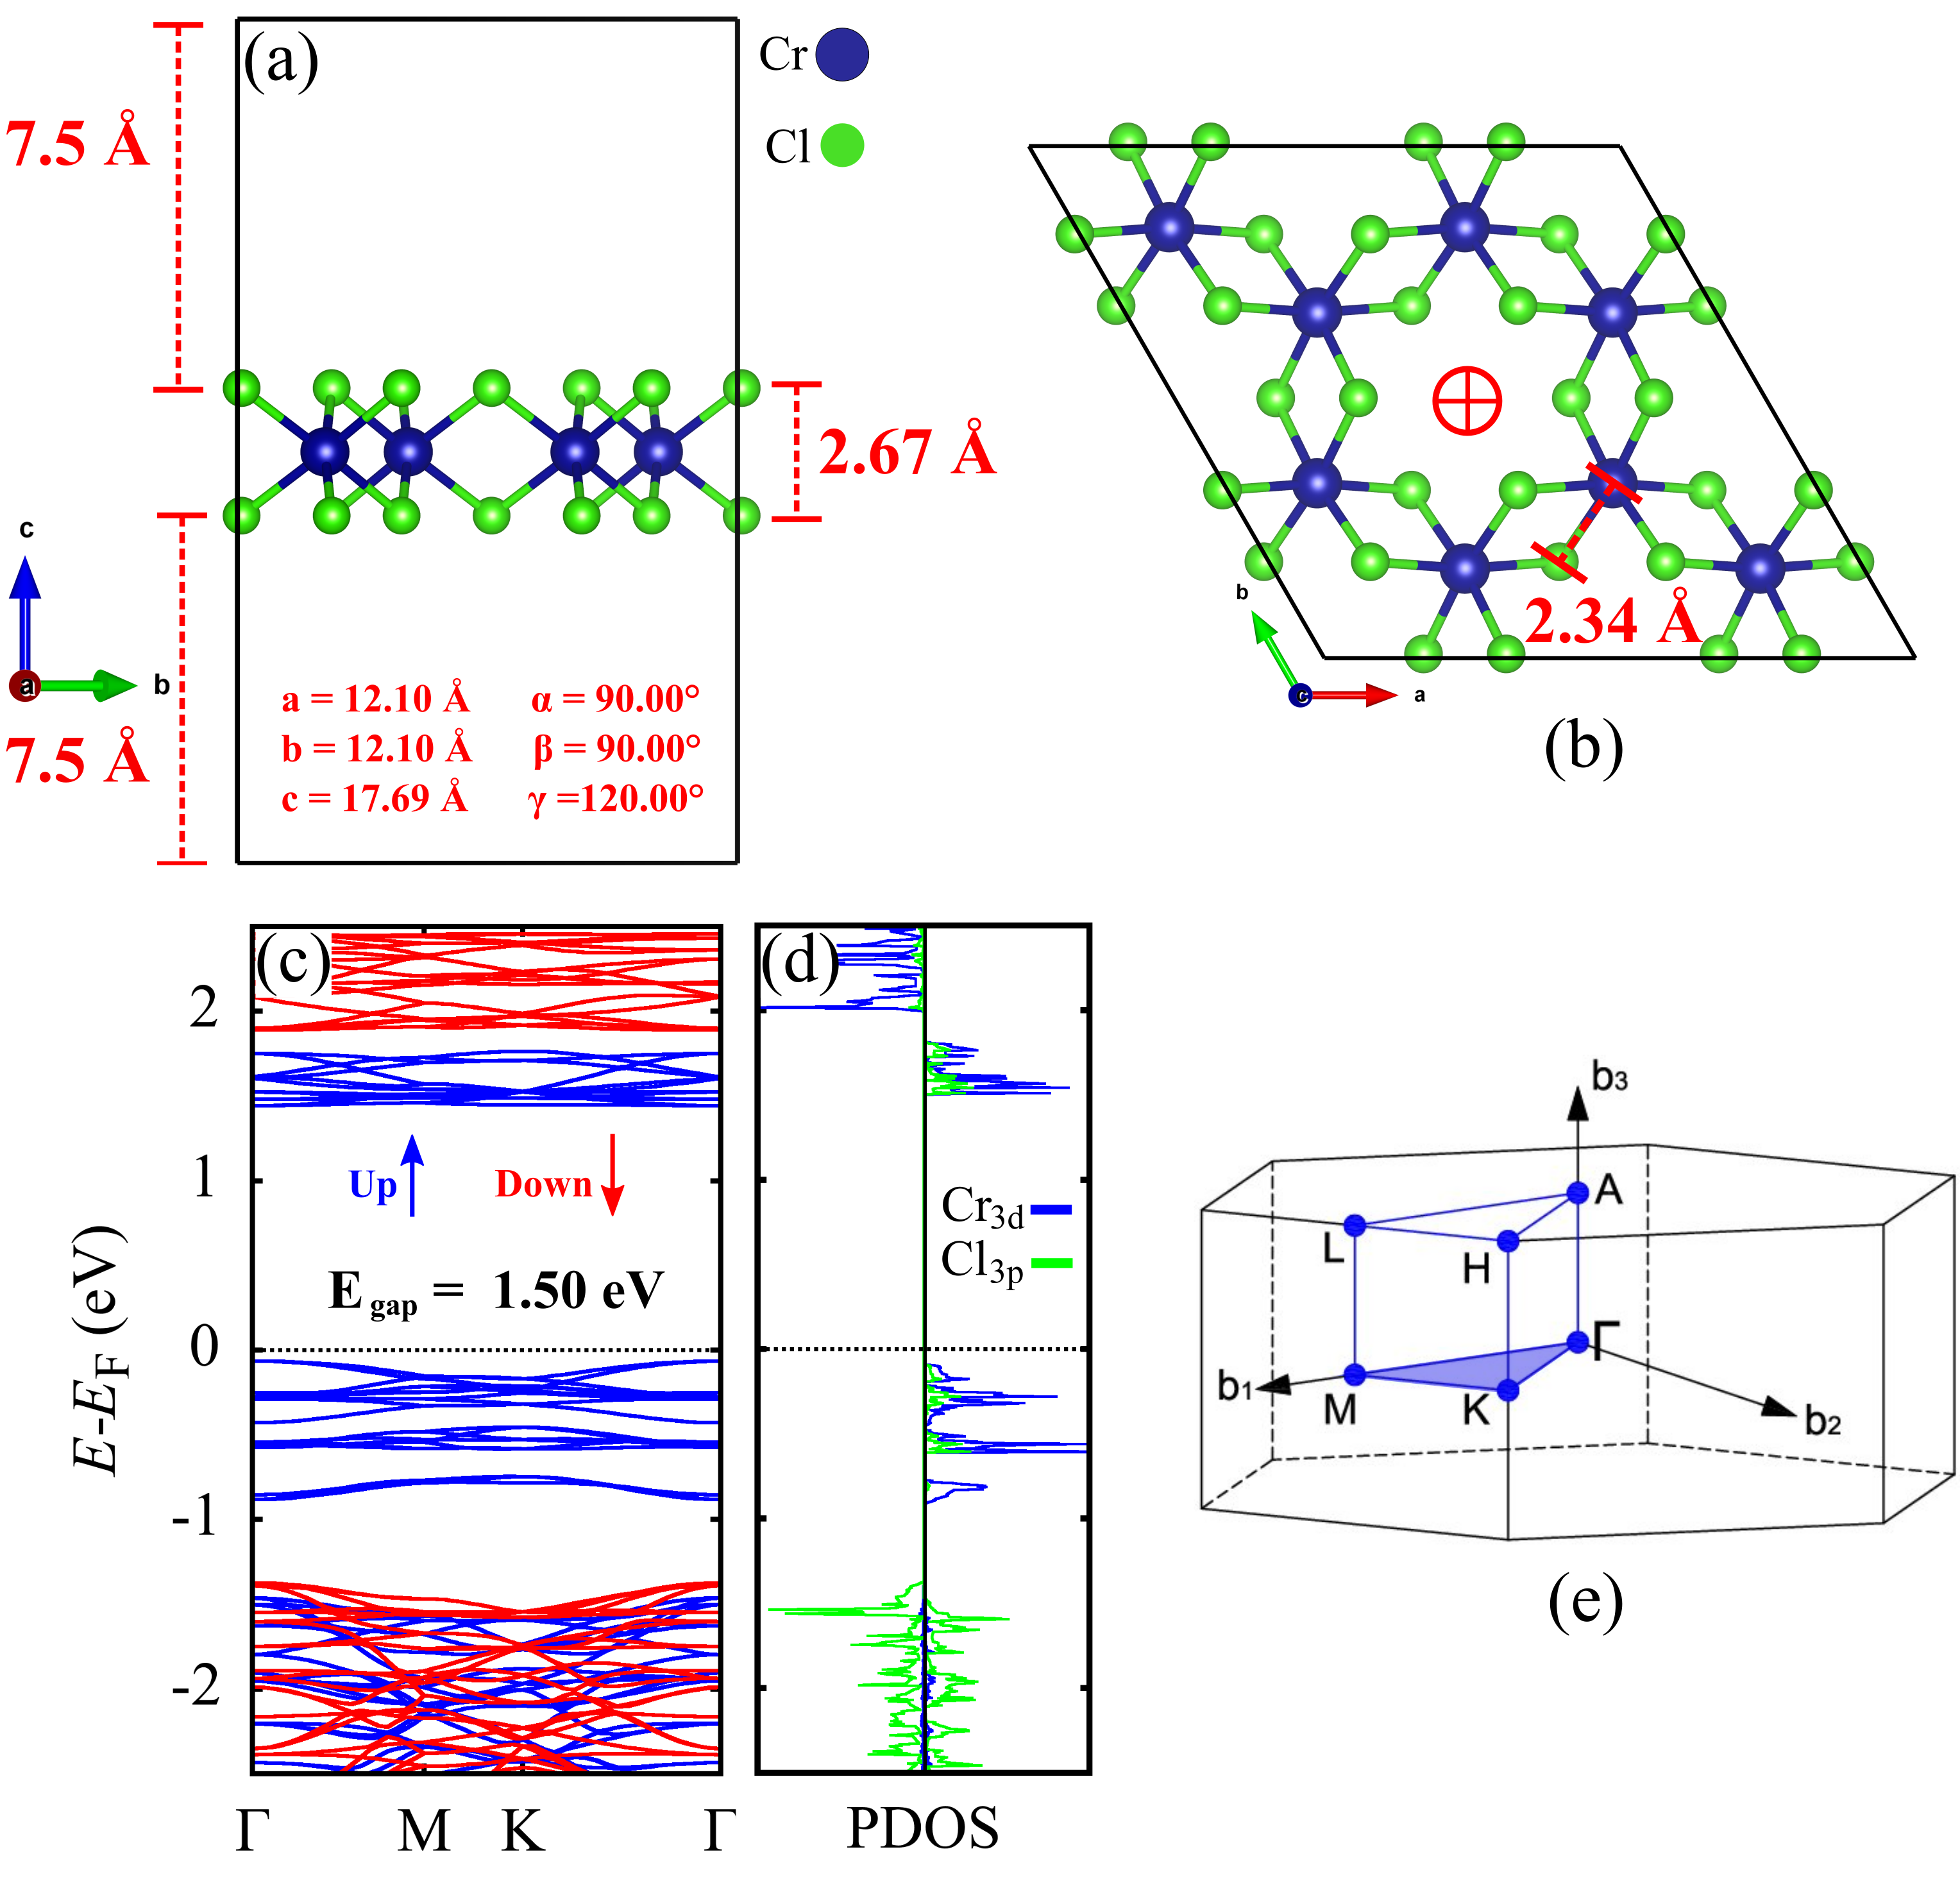
\includegraphics[width=0.8\textwidth]{figure/Fig1.png}
  \caption{Structural, electronic, and magnetic properties of pristine monolayer CrCl$_3$. (a) Side view of the optimized monolayer in the periodic simulation cell, including the lattice parameters, monolayer thickness, and vacuum spacing. (b) Top view showing a representative Cr--Cl bond length and the hollow site considered for transition-metal functionalization. (c) Spin-resolved band structure along $\Gamma$--M--K--$\Gamma$, with the Fermi level set to 0~eV. (d) Projected density of states of the Cr-$3d$ and Cl-$3p$ orbitals. (e) First Brillouin zone and the high-symmetry path used for the band-structure calculations.}
  \label{fig:Fig1}
\end{figure}

The adopted magnetic reference is a collinear ferromagnetic state in which all Cr moments are aligned parallel. The converged Cr$_8$Cl$_{24}$ supercell has a total magnetic moment of 24.0~$\mu_{\mathrm B}$, corresponding to 3.0~$\mu_{\mathrm B}$ per CrCl$_3$ formula unit. The atom-projected moment is approximately 2.935~$\mu_{\mathrm B}$ per Cr atom, whereas each Cl atom carries a small antiparallel induced moment of approximately $-0.031~\mu_{\mathrm B}$. The magnetization is therefore concentrated primarily on the Cr-$3d$ states, with weaker ligand polarization arising from Cr--Cl hybridization. These values are consistent with the expected Cr$^{3+}$ $3d^3$ configuration, corresponding to $S=3/2$, and with previous first-principles calculations reporting local Cr moments close to $3~\mu_{\mathrm B}$ \cite{Gao2018,Mastrippolito2022,Soriano2020}. The weak ligand polarization is also consistent with the established role of Cr-$3d$/Cl-$3p$ hybridization in the magnetic response of CrCl$_3$\cite{Besbes2019}.

Within the present PBE description, pristine CrCl$_3$ is a spin-polarized semiconductor with a direct band gap of 1.50~eV [Figure~\ref{fig:Fig1}(c)], in close agreement with previous spin-polarized GGA-PBE values of approximately 1.6~eV~\cite{Gao2018,Luo2020}. The spin inequivalence of the bands reflects the ferromagnetic Cr sublattice, while the projected density of states in Figure~\ref{fig:Fig1}(d) shows substantial Cr-$3d$ character near the band edges and dominant Cl-$3p$ contributions to the occupied valence manifold, together with appreciable Cr-$3d$/Cl-$3p$ hybridization at lower energies. Within the scope of the present work, this electronic-structure analysis is used primarily to establish the orbital and spin character of the pristine reference system and to provide a consistent basis for comparison with the transition-metal-functionalized configurations, rather than to use the absolute band-gap value as a quantitative descriptor of hydrogen adsorption.

Combined with the chemically saturated, Cl-terminated basal plane, this gapped electronic structure provides limited spatial accessibility to the underlying Cr centers for direct H binding. This electronic and structural picture therefore establishes pristine CrCl$_3$ as the reference system for evaluating how transition-metal functionalization modifies the local adsorption environment.

Hydrogen adsorption on the pristine basal plane was evaluated at the top-Cl ($S_1$), hollow ($S_2$), and top-Cr ($S_3$) sites shown in Figure~\ref{fig:Fig2}(a). After unconstrained relaxation, H initially placed at $S_1$ moves away from the surface, reaching a final H--surface separation of approximately 3.42~\AA, while H initialized at $S_2$ does not remain at the hollow position [Figure~\ref{fig:Fig2}(b,c)]. Neither site therefore yields a locally stable chemisorbed state under the conditions considered.

\begin{figure}[H]
  \centering
  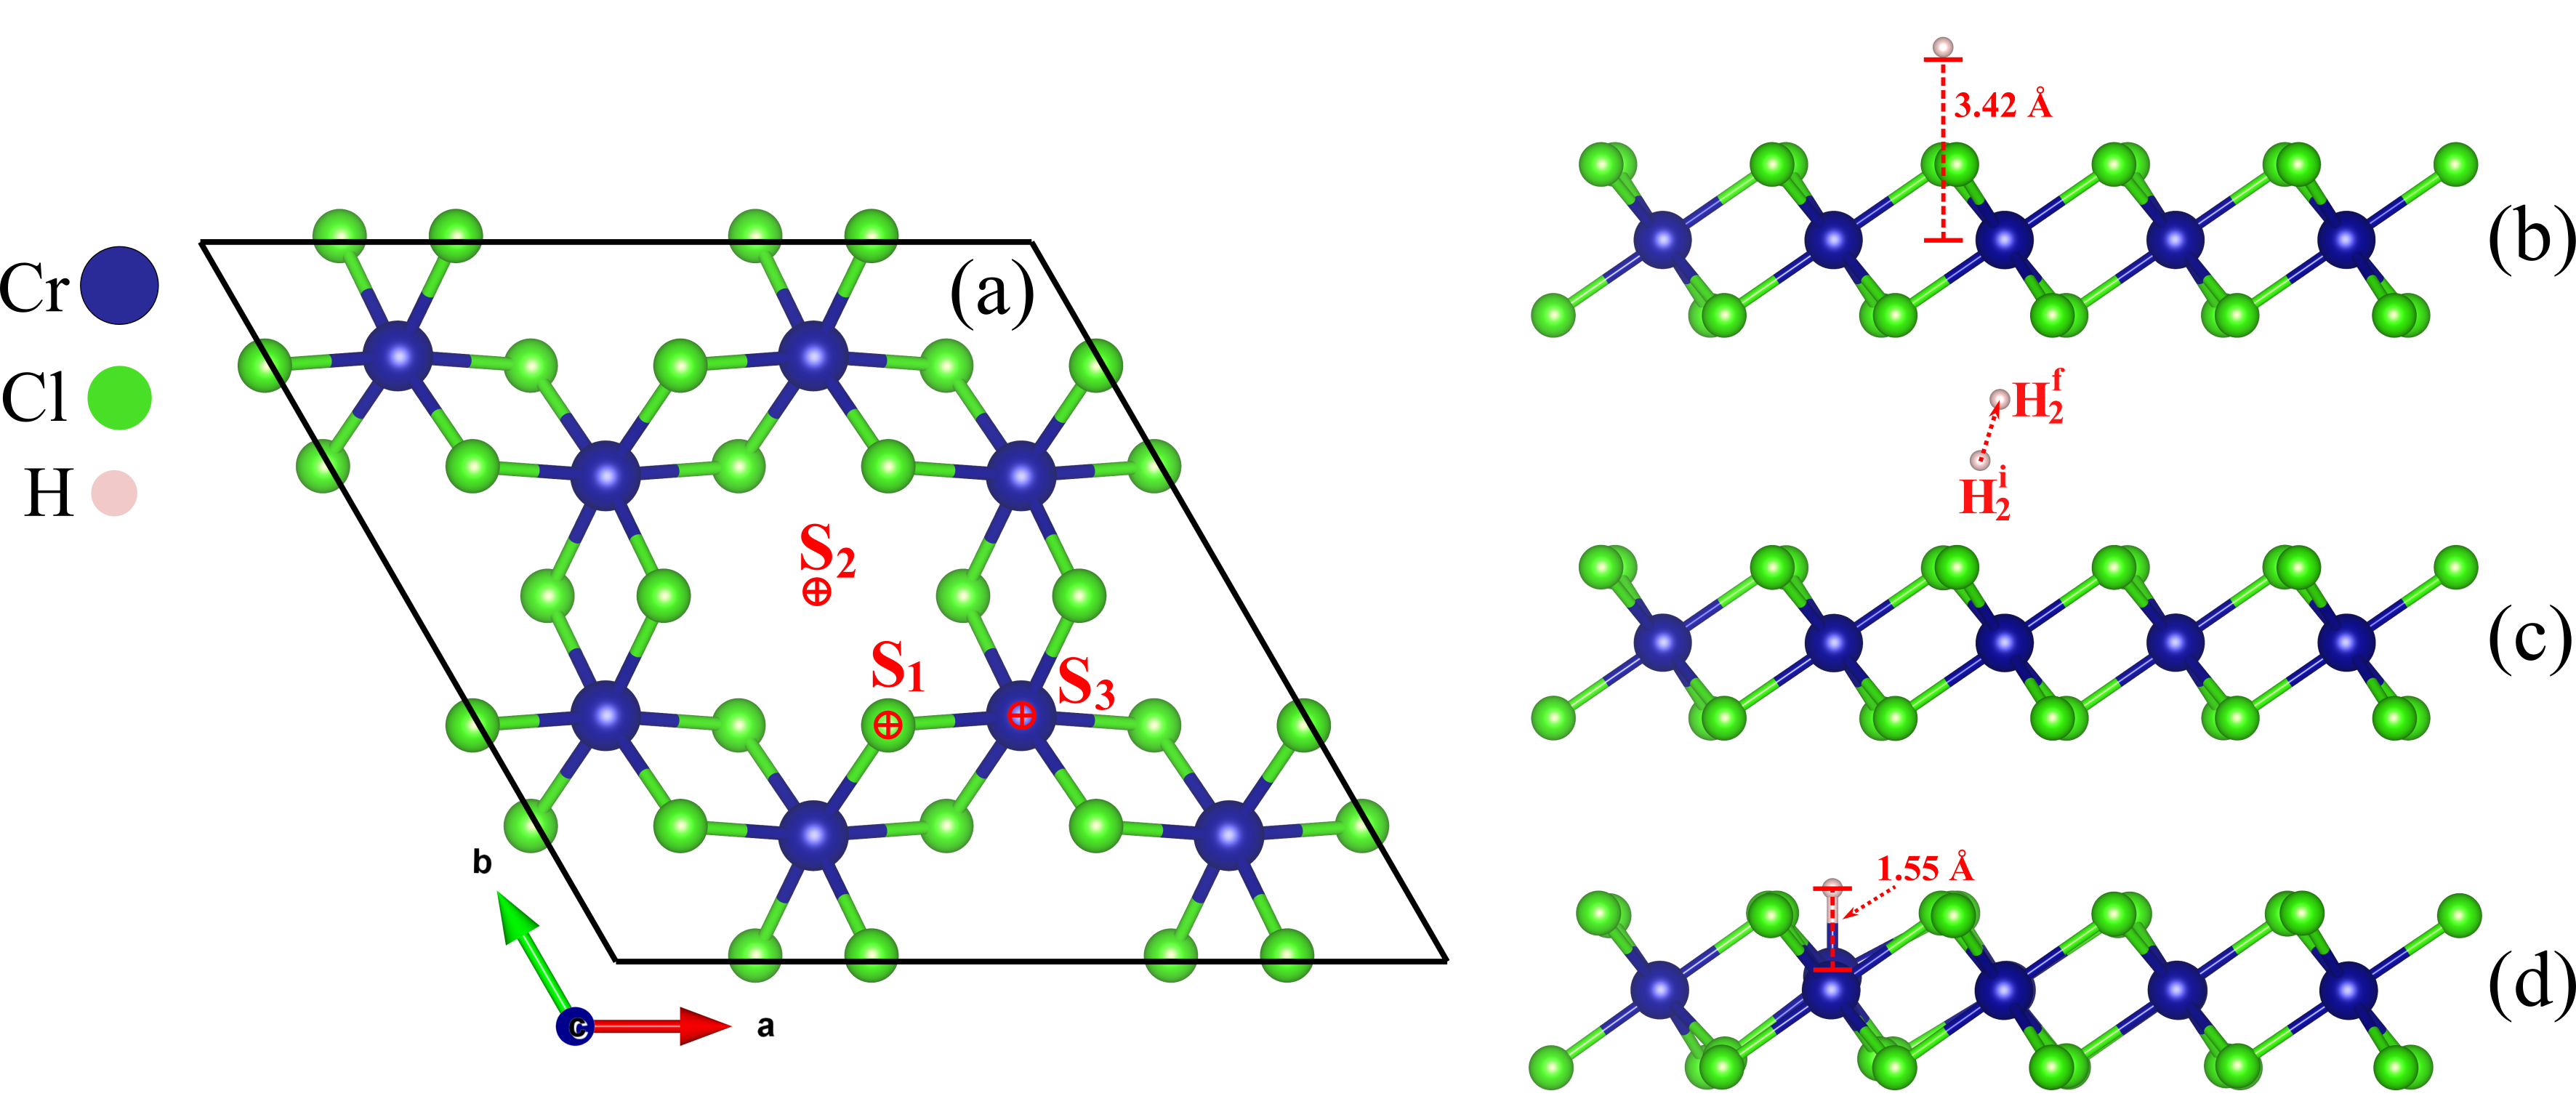
\includegraphics[width=1.0\textwidth]{figure/Fig2.png}
  \caption{Hydrogen adsorption on pristine monolayer CrCl$_3$. (a) Initial top-Cl ($S_1$), hollow ($S_2$), and top-Cr ($S_3$) adsorption sites. (b--d) Relaxed configurations obtained from $S_1$, $S_2$, and $S_3$, respectively. H is not retained at the top-Cl or hollow positions, whereas the top-Cr configuration forms a local H--Cr contact of 1.55~\AA\ but remains thermodynamically unfavorable, with $\Delta G_{\mathrm{ads}}=1.82$~eV.}
  \label{fig:Fig2}
\end{figure}

By contrast, the $S_3$ configuration relaxes to a locally bound geometry with an H--Cr distance of 1.55~\AA\ [Figure~\ref{fig:Fig2}(d)]. The persistence of this configuration upon structural relaxation indicates the existence of a local adsorption minimum. Nevertheless, its adsorption free energy is strongly positive, $\Delta G_{\mathrm{ads}} = 1.82$~eV, showing that H$^*$ formation is highly endergonic relative to the $\frac{1}{2}$H$_2$ reference. At the investigated coverage of one H atom per $2\times2\times1$ supercell, pristine monolayer CrCl$_3$ is consequently an unfavorable host for H$^*$ formation. A previous spin-polarized DFT study reported a much lower hydrogen adsorption free energy (on the order of 0.1~eV) for pristine monolayer CrCl$_3$~\cite{Zala2024}. However, direct comparison is limited by differences in adsorption geometry, coverage, supercell size, basis representation, and relaxation protocol. The two values are not contradictory: our 1.82~eV arises from H binding directly to the Cr center after penetrating the Cl surface layer (top-Cr, $S_3$ site), which is the only locally stable chemisorbed state under our protocol; the near-thermoneutral value of Ref.~\cite{Zala2024} corresponds to a distinct weakly chemisorbed on-Cl or near-Cl configuration at different coverage and computational parameters. Systematic multi-scale supercell calculations across $1\times 1$ ($\theta = 1.0$, $d_{\mathrm{H-H}} \approx 6.05$~\AA), $2\times 2$ ($\theta = 0.25$, $d_{\mathrm{H-H}} \approx 12.09$~\AA), and $3\times 3$ ($\theta = 0.111$, $d_{\mathrm{H-H}} \approx 18.14$~\AA) cells confirm that the chemisorbed $S_3$ site is intrinsically converged ($\Delta G_{\mathrm{ads}} = 1.88, 1.86, 1.84$~eV, varying by only 0.036~eV), while the $S_1$ top-Cl site stabilizes to 1.51~eV in the dilute limit due to long-range lattice compliance. Both results confirm that pristine CrCl$_3$ is not an intrinsically active HER host, motivating transition-metal functionalization.

These results establish the reference behavior of the ideal basal plane: the outer Cl layer restricts access to the Cr-$3d$ centers, and the only locally retained H configuration remains far from thermoneutral adsorption. Transition-metal functionalization is therefore considered as a route to introduce exposed $3d$ centers and modify the local H-binding environment. The present analysis is limited to adsorption thermodynamics and does not address proton-transfer, H-diffusion, or H$_2$-formation barriers.

\subsection{Transition-metal functionalization: local coordination and finite-temperature behavior}

\noindent The hollow region highlighted in Figure~\ref{fig:Fig1}(b) provides two chemically distinct coordination motifs and has previously been identified as an accessible adsorption region for Li and O on monolayer CrCl$_3$~\cite{Luo2020,Mastrippolito2022}. In the surface-adsorbed geometry, the transition-metal atom remains exposed above the monolayer and interacts primarily with three Cl neighbors, whereas in the embedded geometry it penetrates the Cl-terminated surface and becomes coordinated by Cl atoms from both sides of the layer. This comparison isolates the effect of increased TM--Cl coordination and reduced geometrical exposure of the metal center.

The optimized surface-adsorbed structures are shown in Figure~\ref{fig:Fig3}(a--c). Co, Fe, and Ni remain anchored at the hollow region without global reconstruction of the CrCl$_3$ framework. Their vertical distances from the average Cr plane are 1.92, 1.76, and 1.44~\AA, respectively, establishing a progressive reduction in site exposure from Co to Ni. The corresponding atom-referenced binding energies are $-2.82$, $-2.60$, and $-3.38$~eV. Ni therefore combines the deepest accommodation with the strongest local interaction with the substrate, whereas Co and Fe remain more exposed while retaining favorable anchoring.

\begin{figure}[H]
  \centering
  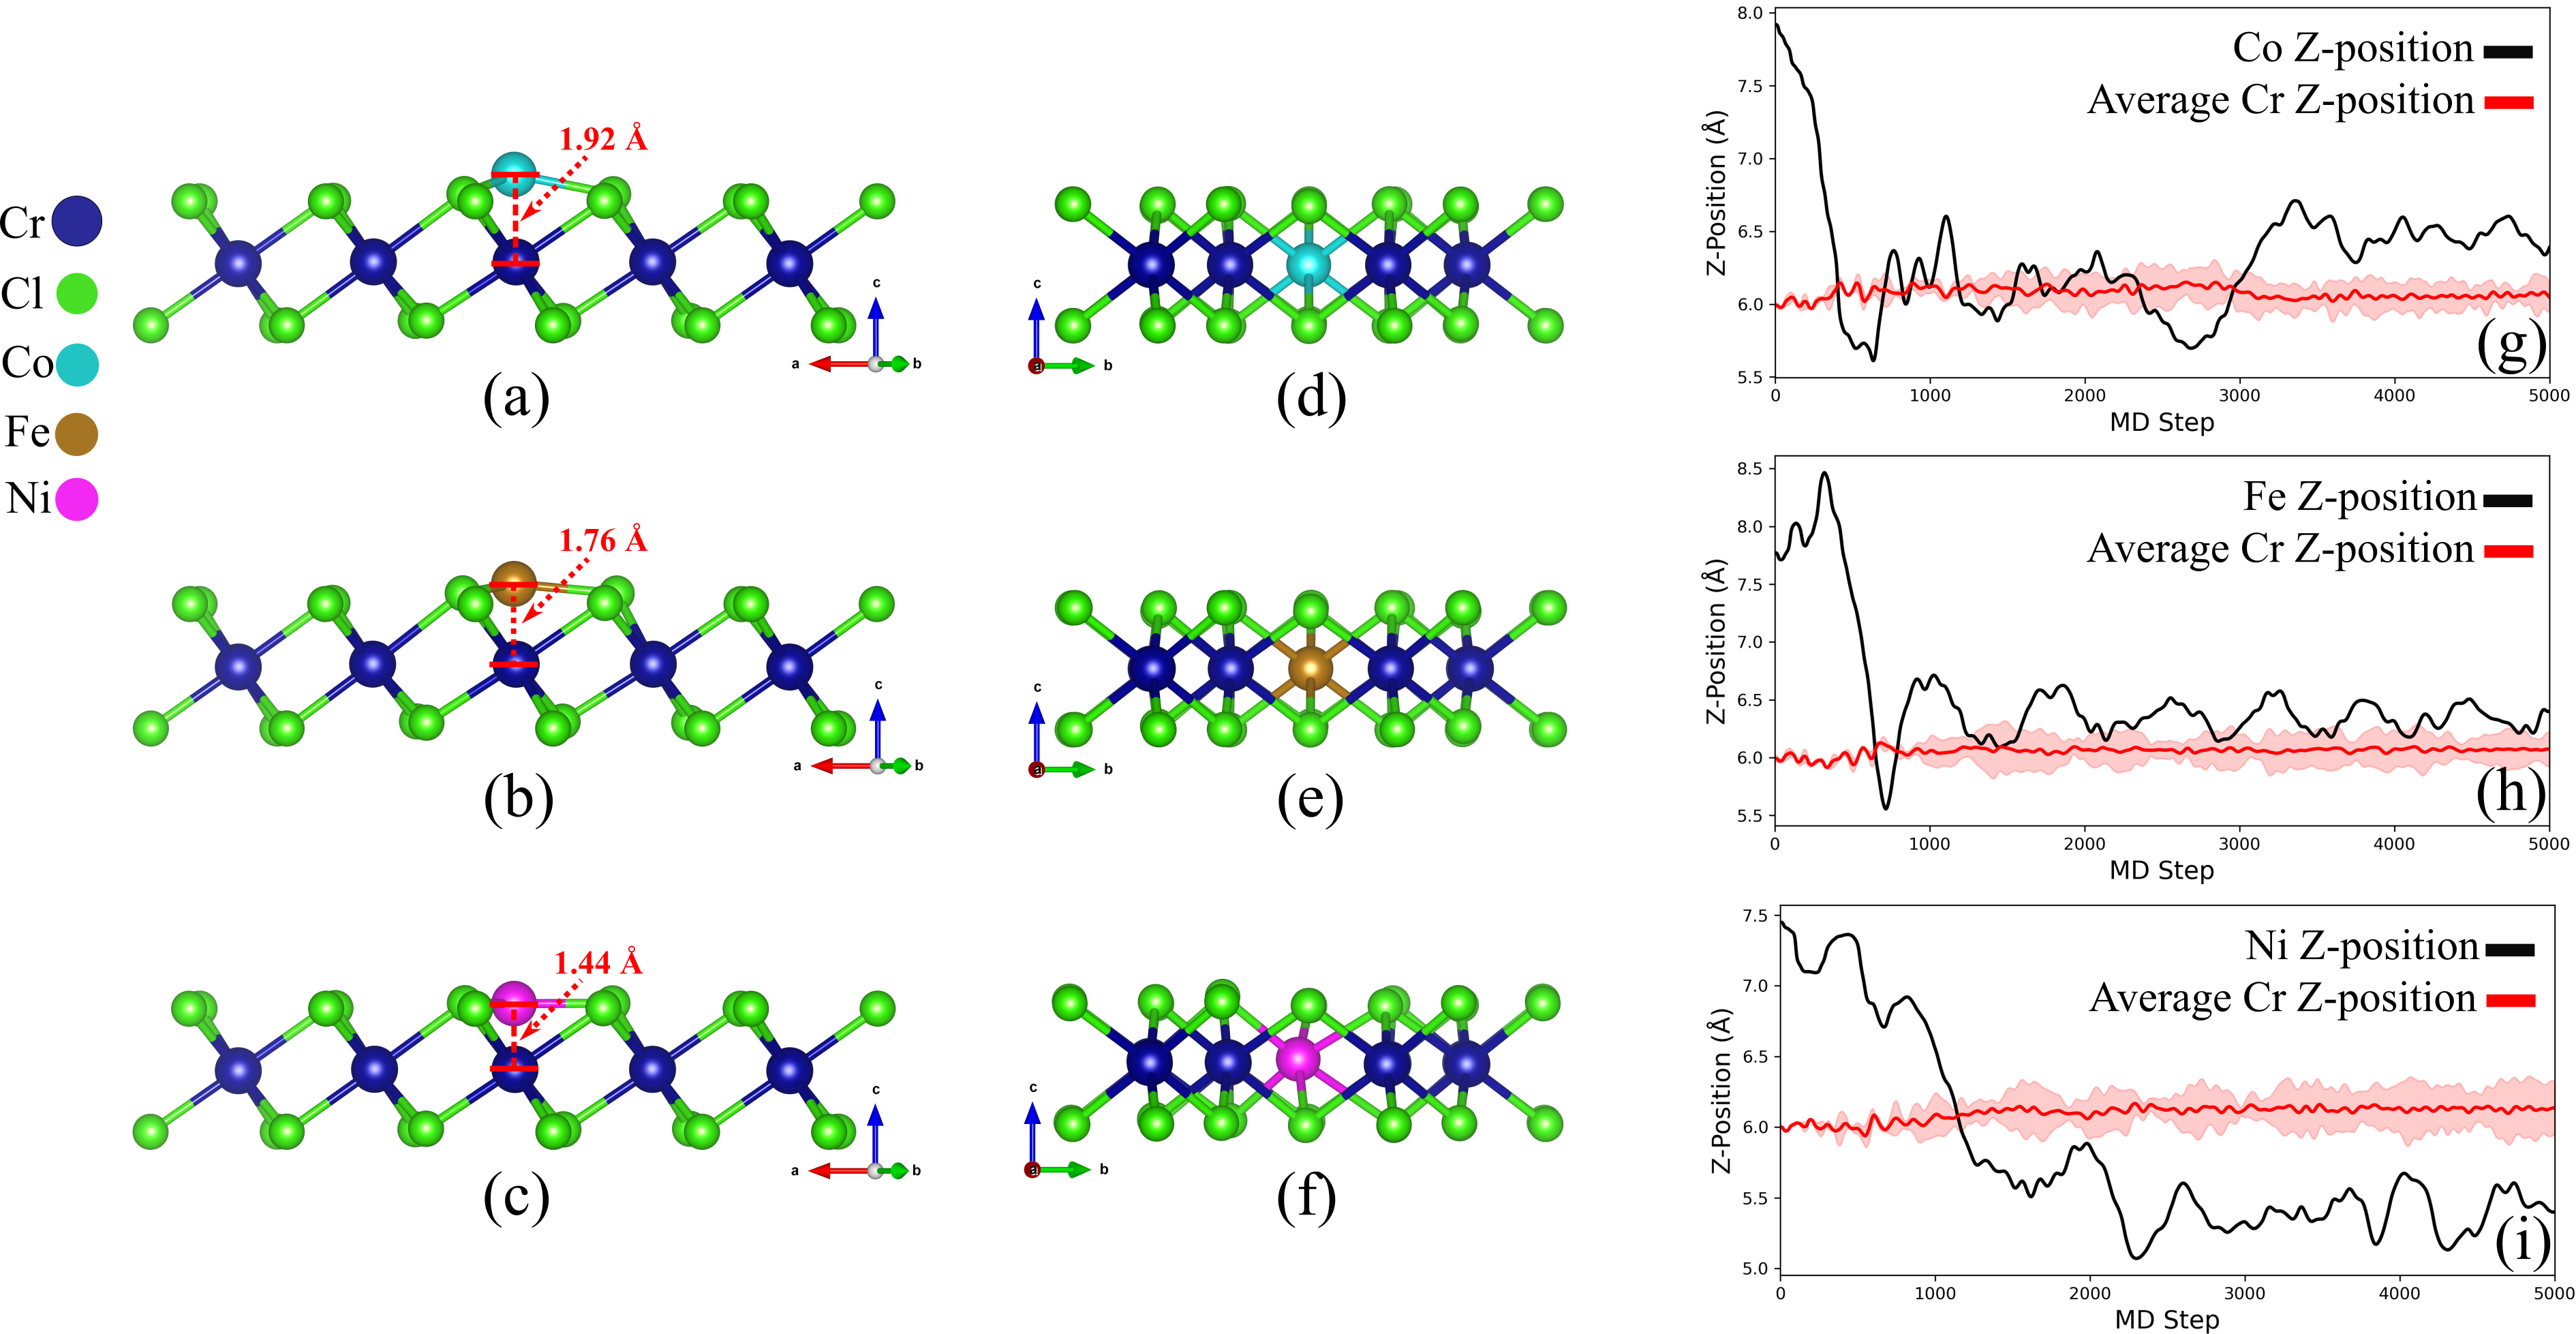
\includegraphics[width=1.0\textwidth]{figure/Fig3.png}
  \caption{Structural configurations and finite-temperature evolution of Co-, Fe-, and Ni-functionalized monolayer CrCl$_3$. (a--c) Optimized surface-adsorbed configurations, with the vertical TM--Cr-plane distances indicated. (d--f) Corresponding embedded configurations. (g--i) Absolute TM $z$ coordinates during 5~ps AIMD simulations at 300~K. Black curves denote the transition-metal positions; red curves and shaded regions represent the average Cr-plane position and its fluctuations.}
  \label{fig:Fig3}
\end{figure}

These binding energies quantify local TM--CrCl$_3$ bond formation relative to isolated spin-polarized transition-metal atoms. Comparing $|E_{\mathrm{bind}}|$ to the PBE cohesive energies of the bulk metals (Co: 4.39~eV/atom; Fe: 4.28~eV/atom; Ni: 4.44~eV/atom) reveals that only embedded Ni ($|E_{\mathrm{bind}}| = 4.95$~eV) is thermodynamically stable against bulk-metal formation. For the adsorbed configurations and Co/Fe-embedded, the cohesive energy of the bulk metal exceeds $|E_{\mathrm{bind}}|$ by 0.3--2.1~eV, meaning that aggregation into metal clusters is thermodynamically downhill relative to the isolated-atom reference. This is a known limitation of isolated-atom DFT binding energies and is common to the SAC literature. In practice, isolated Co and Fe surface sites are kinetically stabilized by the energy barrier required to migrate through the constrained CrCl$_3$ hollow region -- a barrier that prevents room-temperature aggregation within the 5~ps AIMD window. These binding energies do not, by themselves, establish stability against metal clustering or bulk-metal formation and should not be interpreted as a complete thermodynamic assessment of isolated-site dispersion.

The charge-density-difference isosurfaces in Figure~\ref{fig:Fig4}(a--c) show localized charge redistribution around the transition-metal centers and neighboring Cl atoms. The TM atoms act as electron donors: Co, Fe, and Ni each transfer electrons to the CrCl$_3$ substrate, with Bader-integrated charge transfers of $\Delta Q = 0.77$, $0.94$, and $0.59~e$, respectively [Figure~\ref{fig:Fig4}(d--f)]. The positive Bader charge variation ($\Delta Q > 0$) on the TM center and the corresponding electron accumulation on adjacent Cl atoms (visible as red regions in the charge-difference maps) confirm this donor character. Although Fe exhibits the largest charge transfer, Ni has the most negative binding energy, indicating that metal--substrate stabilization depends not only on charge redistribution but also on the spatial and energetic hybridization of TM-$3d$, Cr-$3d$, and Cl-$3p$ states. This interpretation is consistent with previous studies emphasizing adsorption-induced changes in Cl-$3p$/Cr-$3d$ hybridization and the broader role of ligand-$p$ states in the electronic and magnetic coupling of chromium trihalides~\cite{Luo2020,Besbes2019}.

\begin{figure}[H]
  \centering
  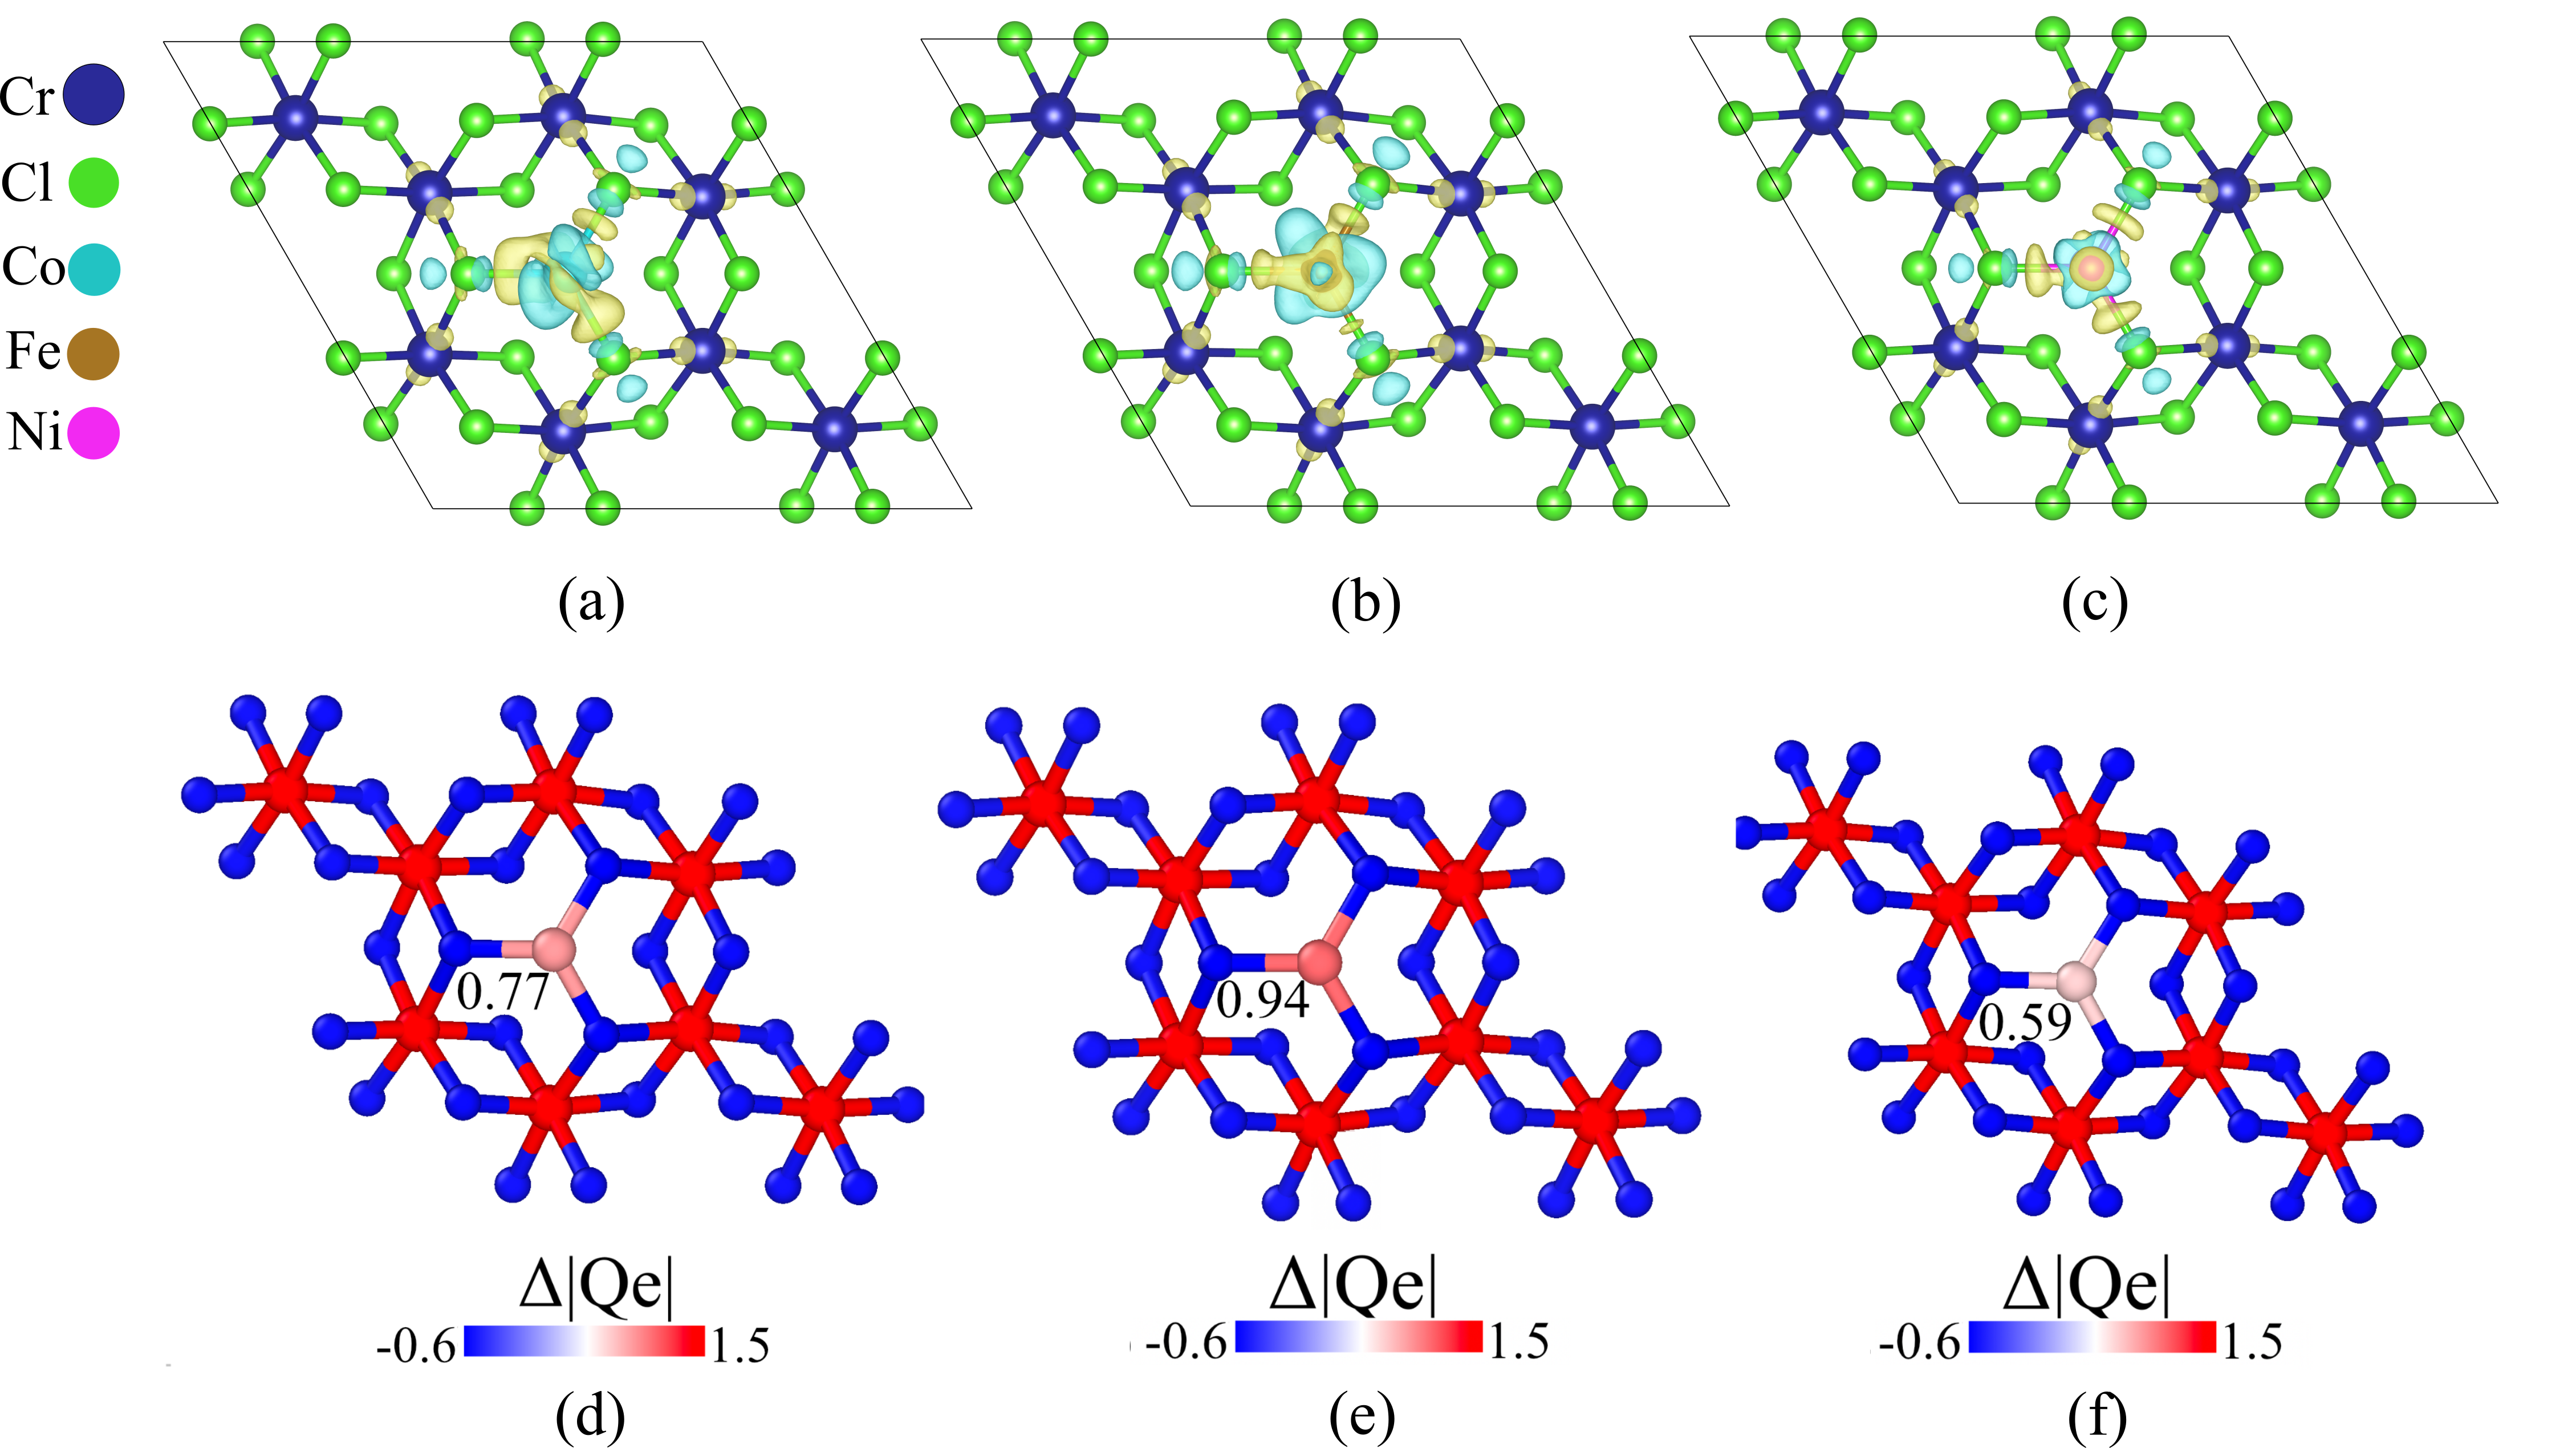
\includegraphics[width=1.0\textwidth]{figure/Fig4.png}
  \caption{Charge redistribution induced by transition-metal adsorption on monolayer CrCl$_3$. (a--c) Charge-density-difference isosurfaces for surface-adsorbed Co, Fe, and Ni, plotted at $\delta=5\times10^{-3}$~$e$/\AA$^{3}$. (d--f) Corresponding Bader charge-variation maps. Blue and red regions denote electron depletion and accumulation, respectively; the numerical labels indicate the charge-transfer magnitude associated with each transition-metal atom.}
  \label{fig:Fig4}
\end{figure}

The functionalizing metals also generate distinct local spin states. The atom-projected moments of surface-adsorbed Co, Fe, and Ni are $1.99$, $3.34$, and $-0.76~\mu_{\mathrm B}$, respectively, where the positive direction is defined by the Cr sublattice. Co and Fe are therefore polarized parallel to the ferromagnetic host, whereas Ni is antiparallel. The magnetic response is consequently metal dependent, although its relevance to H adsorption must be evaluated together with coordination, orbital occupation, and structural relaxation.

The embedded structures in Figure~\ref{fig:Fig3}(d--f) adopt distorted sixfold environments that are approximately octahedral, as detailed in Figure~S1. Their atom-referenced binding energies are $-3.55$, $-3.36$, and $-4.95$~eV for Co, Fe, and Ni, respectively. Relative to the threefold surface geometries, the additional Cl neighbors provide a larger coordination shell and more extensive incorporation into the Cr--Cl framework. The corresponding local moments are $2.09$, $3.34$, and $-1.02~\mu_{\mathrm B}$. Embedding only weakly changes the Co and Fe moments but increases the magnitude of the antiparallel Ni polarization.

The strongly metal-dependent local spin response is consistent with earlier transition-metal-doping studies, in which Ni and Mo incorporation produced substantial changes in the spin-resolved electronic structure, magnetic coupling, and local moments of CrCl$_3$\cite{Wang2019,Safi2023}.

The persistence of the surface-adsorbed motifs at finite temperature was examined by 5~ps AIMD simulations at 300~K. Co undergoes an initial vertical relaxation and then fluctuates predominantly above the average Cr plane [Figure~\ref{fig:Fig3}(g)]. Fe exhibits a similar adjustment and remains slightly surface exposed [Figure~\ref{fig:Fig3}(h)]. No rapid vertical desorption is observed for either metal within the simulated time window.

Ni behaves differently: its vertical coordinate decreases continuously during the early trajectory, crosses the average Cr plane, and subsequently fluctuates within the monolayer interior [Figure~\ref{fig:Fig3}(i)]. The analogous trajectory of an additional Cr atom in Figure~S2 supports the interpretation that this motion represents loss of surface exposure and incipient incorporation rather than ordinary vibrations around the initial adsorption height. The temperature profiles in Figure~S3 fluctuate around 300~K after the initial thermostatting transient, indicating that the contrasting TM trajectories are sampled under comparable thermal conditions.

The static and dynamical calculations therefore consistently establish the stability hierarchy of the two coordination motifs. Embedded configurations are thermodynamically favored at 0~K for all three metals ($\Delta E_{\mathrm{emb-ads}}^{\mathrm{TM}} < 0$), with Ni displaying the strongest incorporation driving force ($-1.57$~eV) and spontaneous penetration from the surface into the embedded position during the 300~K AIMD trajectory [Figure~\ref{fig:Fig3}(i)], directly confirming the dynamic accessibility and stability of the embedded motif. Conversely, surface-adsorbed Co and Fe remain kinetically trapped in the surface state at 300~K over 5~ps [Figure~\ref{fig:Fig3}(g,h)], which is essential for preserving the exposed, near-thermoneutral active sites required for HER electrocatalysis. The trajectories thus reveal short-time structural accessibility while confirming that both coordination motifs are dynamically stable against lattice degradation or thermal desorption.

\subsection{Coordination-dependent electronic structure and TM--Cl bonding}

\noindent Figure~\ref{fig:Fig5} shows that transition-metal functionalization introduces spin-polarized states within or near the gap of pristine CrCl$_3$, consistent with previous calculations of Cr and Cl vacancies, surface oxidation, and transition-metal substitution in CrCl$_3$ \cite{Gao2018,Mastrippolito2021,Wang2019,Safi2023}. These features contain substantial TM-$3d$ character and overlap with the Cr-$3d$ and Cl-$3p$ manifolds. Their generally weak dispersion indicates localization around the functionalizing center, whereas their hybrid character confirms electronic coupling to the host rather than the formation of isolated atomic levels.

For the surface-adsorbed systems [Figure~\ref{fig:Fig5}(a--f)], Co and Fe generate narrow TM-derived states at or near the Fermi level while largely preserving the broader CrCl$_3$ valence and conduction manifolds. Ni produces a stronger rearrangement of the in-gap spectrum, including several occupied, weakly dispersive Ni-$3d$ states and a more pronounced modification of the host band-edge region. This trend is consistent with its lower adsorption height and stronger atom-referenced binding to the substrate.

  Embedding reorganizes the TM-$3d$ manifold through the structural transition from threefold surface adsorption to distorted sixfold hollow coordination [Figure~\ref{fig:Fig5}(g--l)]. This coordination change manifests in three distinct spectral features: (i)~\textit{Spectral redistribution and enhanced crystal-field splitting}: while surface-adsorbed Co exhibits a single predominant TM-$3d$ feature near $E_{\mathrm F}$ [Figure~\ref{fig:Fig5}(b)], embedded Co displays multiple distinct narrow peaks spread over a wider energy window ($\sim$$-5$ to $-1$~eV) [Figure~\ref{fig:Fig5}(h)] due to the higher ligand-field splitting imposed by the six surrounding Cl ligands~\cite{Soriano2020,Nharangatt2022}. (ii)~\textit{Depletion of TM-$3d$ density of states at $E_{\mathrm F}$}: embedded Co and Ni show substantially fewer TM-$3d$ states at the Fermi level compared to their surface counterparts, directly reducing the orbital availability for frontier TM--H $\sigma$-bonding and explaining the attenuated H-interaction energy ($E_{\mathrm{int}}^{\mathrm H} = -0.94$~eV for embedded vs. $-2.46$~eV for surface Co). (iii)~\textit{Enhanced TM-$3d$/Cl-$3p$ hybridization}: the embedded DOS profiles exhibit extensive spectral overlap with the host Cl-$3p$ valence band between $\sim$$-6$ and $-2$~eV [see also corresponding COHP in Figure~\ref{fig:Fig6}], reflecting deeper covalent incorporation of the metal into the CrCl$_3$ framework. Such coordination-induced reorganization of the TM-$3d$ manifold is consistent with ligand-field arguments and with previous calculations showing that reduced coordination at CrCl$_3$ edges and transition-metal substitution modify the ordering and occupation of the spin-resolved $d$ states~\cite{Wang2019,Safi2023}. Nevertheless, neither the extent of host reconstruction nor the presence of residual states near $E_{\mathrm F}$ alone anticipates the catalytic sequence: embedded Ni perturbs the substrate most strongly but yields an unfavorable adsorption free energy ($\Delta G_{\mathrm{ads}} = 3.62$~eV) due to strong deformation penalties and site blockage.

\begin{figure}[H]
  \centering
  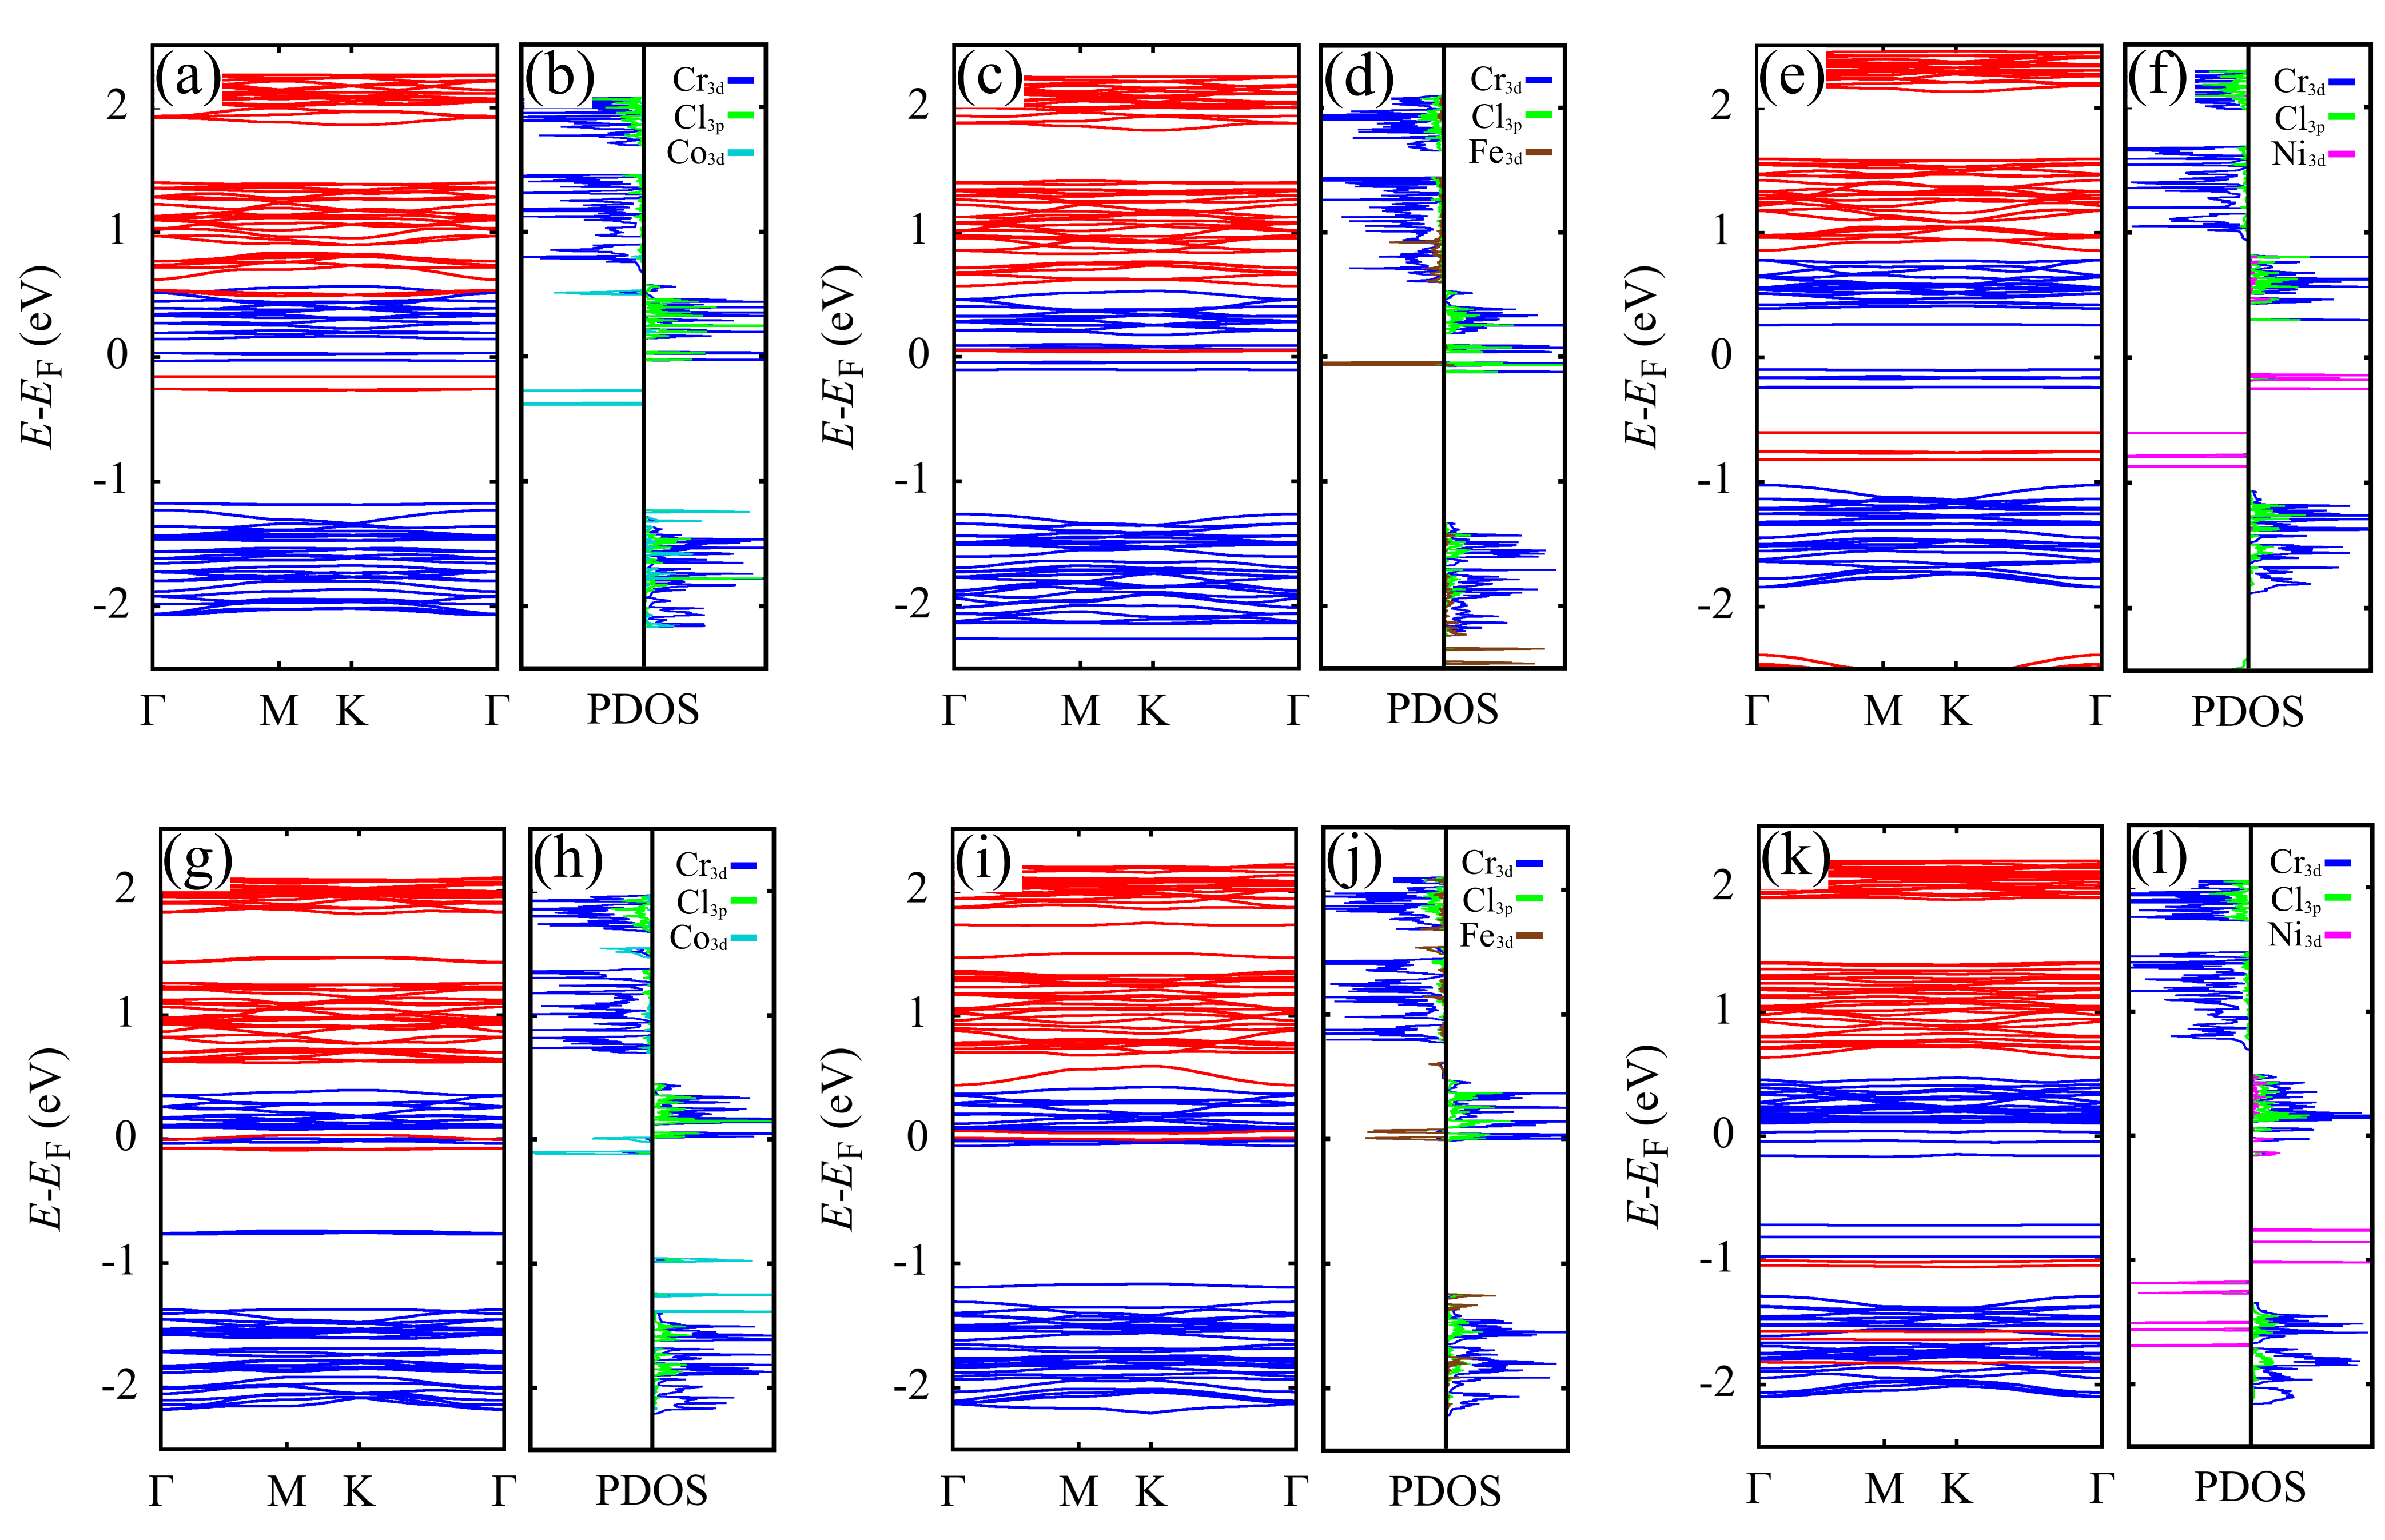
\includegraphics[width=1.0\linewidth]{figure/Fig5.png}
  \caption{Spin-resolved band structures and projected densities of states of transition-metal-functionalized monolayer CrCl$_3$. Panels (a,b), (c,d), and (e,f) correspond to surface-adsorbed Co, Fe, and Ni, respectively; panels (g,h), (i,j), and (k,l) correspond to the embedded configurations. Blue and red bands denote the spin-up and spin-down channels. The PDOS includes Cr-$3d$, Cl-$3p$, and TM-$3d$ contributions, and all energies are referenced to the corresponding Fermi level.}
  \label{fig:Fig5}
\end{figure}

The chemical origin of TM anchoring is resolved by the $-\mathrm{COHP}$ curves in Figure~\ref{fig:Fig6}. For all metals, the dominant occupied bonding manifold extends approximately from $-6.8$ to $-2.5$~eV, coinciding with the TM-$3d$/Cl-$3p$ overlap identified in the PDOS. The metal centers are therefore incorporated into the Cr--Cl framework through covalent orbital hybridization in addition to electrostatic charge redistribution.

\begin{figure}[H]
  \centering
  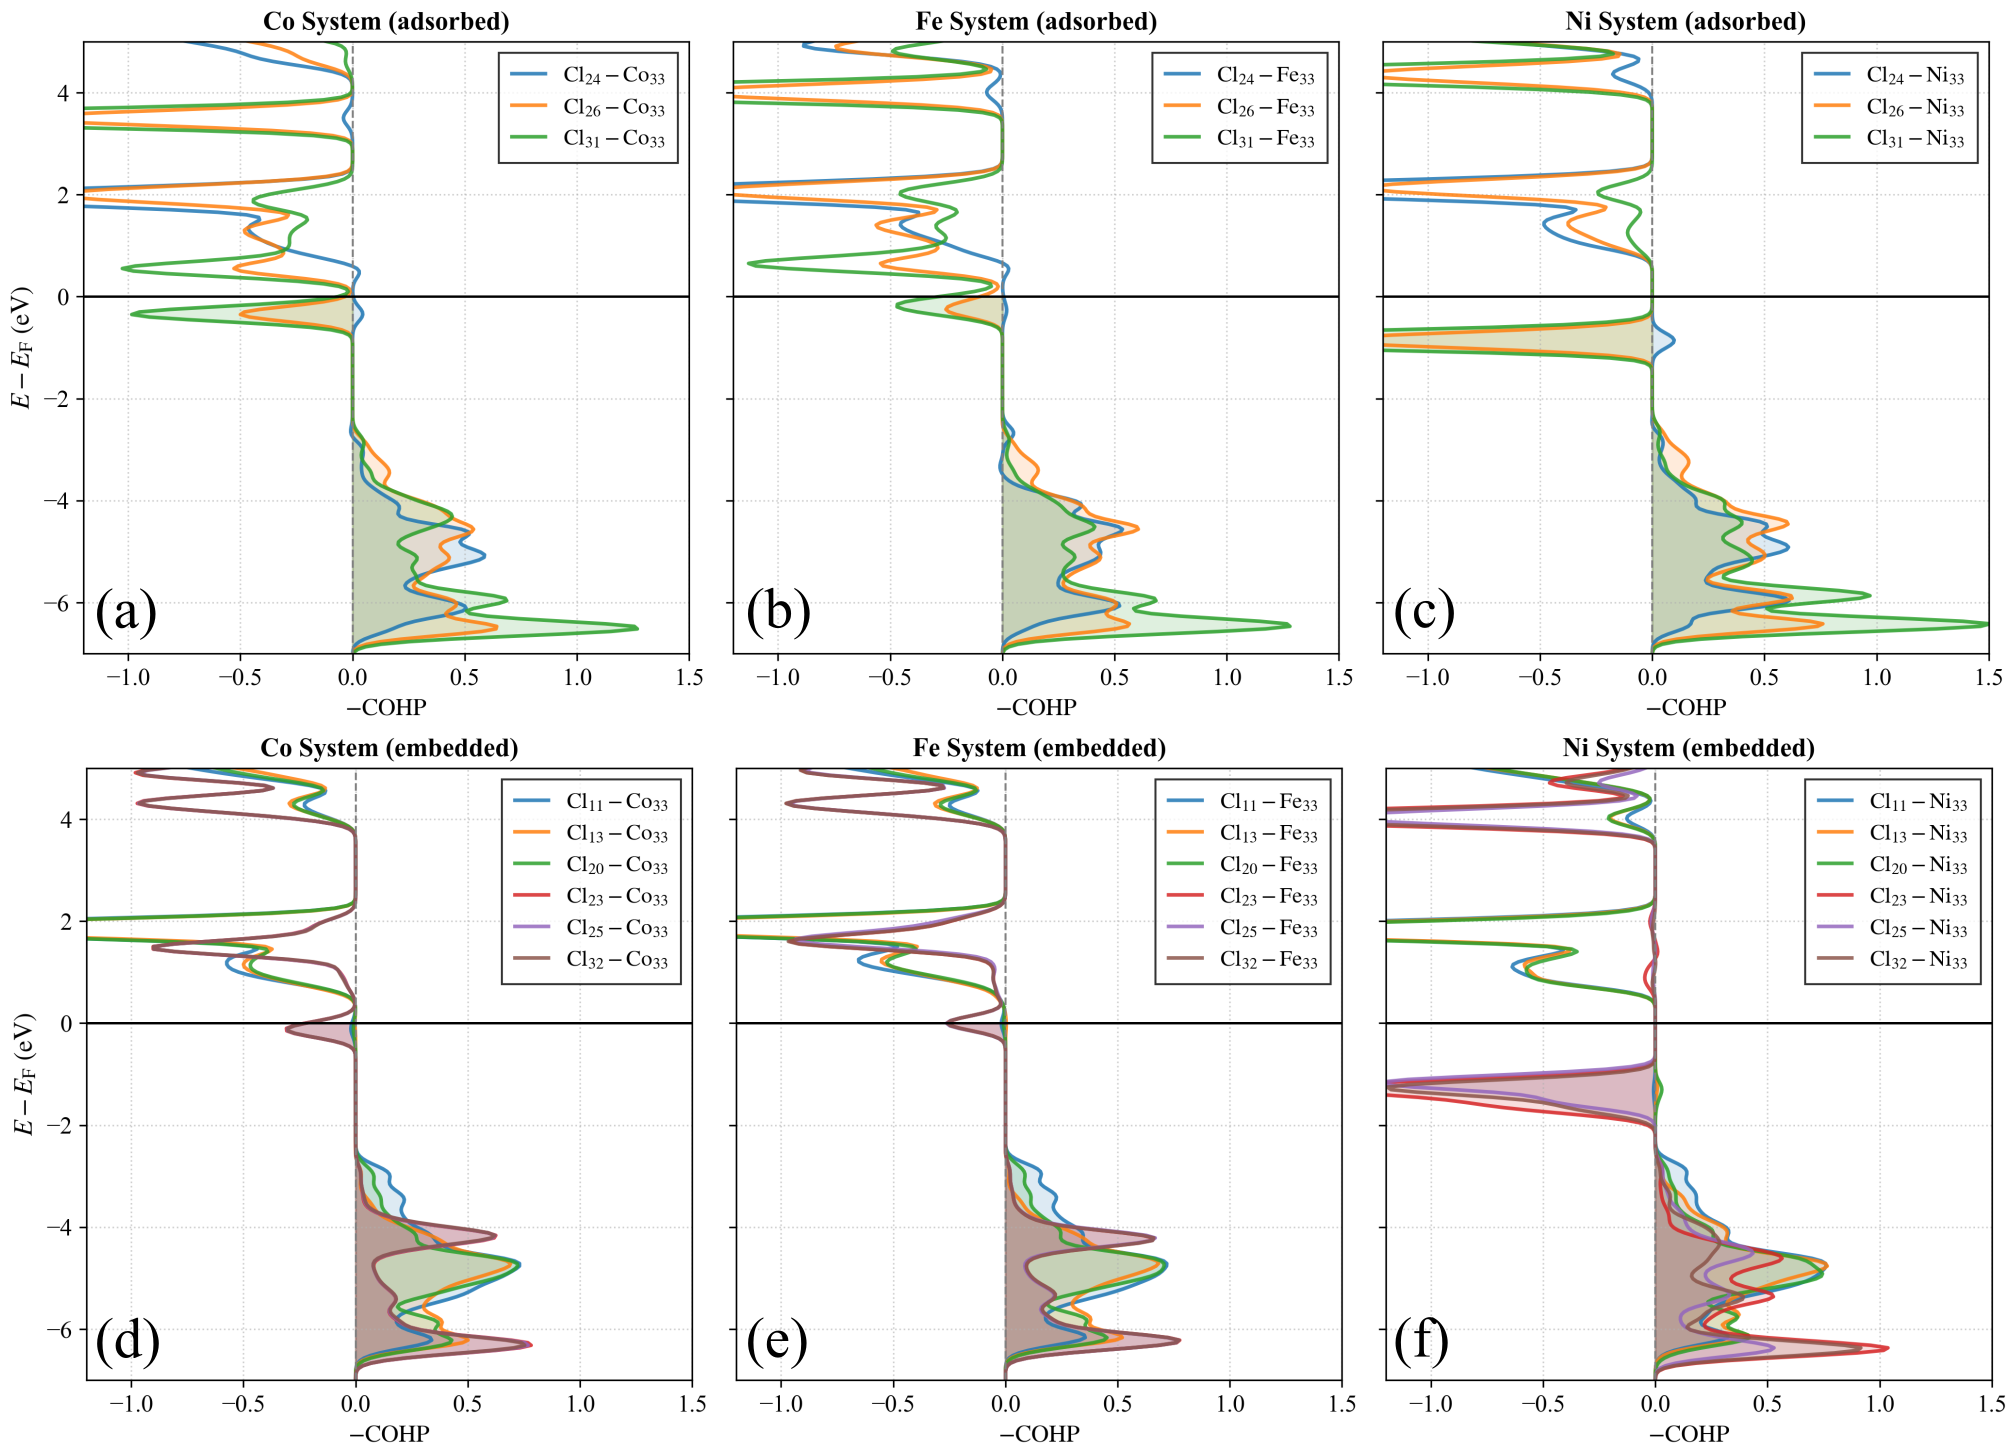
\includegraphics[width=1.0\linewidth]{figure/Fig6.png}
  \caption{Energy-resolved $-\mathrm{COHP}$ curves for individual TM--Cl bonds in transition-metal-functionalized monolayer CrCl$_3$. (a--c) Surface-adsorbed Co, Fe, and Ni in threefold coordination. (d--f) Embedded Co, Fe, and Ni in distorted sixfold coordination. The horizontal line marks the Fermi level. Positive $-\mathrm{COHP}$ values denote bonding contributions and negative values denote antibonding contributions.}
  \label{fig:Fig6}
\end{figure}

In the threefold surface geometries, Co--Cl and Fe--Cl interactions are predominantly bonding at low energies, with comparatively small antibonding contributions near $E_{\mathrm F}$. Surface-adsorbed Ni retains substantial low-energy bonding character but exhibits more pronounced occupied antibonding weight close to the Fermi level. In the embedded structures, distortion of the sixfold environment separates the TM--Cl interactions into nonequivalent groups. This effect is most evident for Ni, where several bonds exhibit appreciable occupied antibonding contributions between approximately $-2$ and $-1$~eV. Increasing coordination therefore redistributes the bonding over a larger, chemically heterogeneous shell rather than uniformly strengthening every TM--Cl contact.

The integrated values in Figure~S4 quantify this distinction. The average ICOHP values per bond are $-2.23$, $-2.28$, and $-2.06$~eV for surface-adsorbed Co, Fe, and Ni, but $-1.87$, $-1.90$, and $-1.67$~eV for the corresponding embedded configurations. Individual TM--Cl bonds are thus stronger on average in the threefold surface motifs. The cumulative ICOHP values, however, become more negative upon embedding, changing from $-6.70$, $-6.84$, and $-6.18$~eV to $-11.22$, $-11.40$, and $-10.01$~eV for Co, Fe, and Ni, respectively. The larger cumulative contribution of the embedded structures originates from the doubled coordination number, not from stronger individual bonds.

Ni has the most negative total binding energy within each coordination family despite the least negative average and cumulative ICOHP values.

This apparent discrepancy is not contradictory because ICOHP isolates the orbital-resolved contributions of selected nearest-neighbor TM--Cl pairs, whereas the total binding energy also contains structural relaxation, electrostatic redistribution, magnetic polarization, and interactions with the wider CrCl$_3$ lattice. The combined analyses therefore establish a coordination trade-off: surface centers form fewer but individually stronger TM--Cl contacts, while embedded centers distribute the interaction over six weaker bonds. This increased integration into the host can stabilize the metal center while reducing its geometrical and orbital availability for bonding with H.

The semiconducting nature of pristine CrCl$_3$ (PBE gap $\sim$1.50~eV; experimental gap $\sim$3~eV) is a practical consideration for electrocatalytic applications. The TM-derived in-gap states shown in Figure~\ref{fig:Fig5} are weakly dispersive and spatially localized around the functionalizing center, and they do not form a percolating conduction channel at the dilute dopant concentration modeled here (one TM per $2\times2\times1$ supercell). Practical implementation would therefore require a conducting support electrode (e.g., carbon cloth, graphene, or glassy carbon) to deliver electrons to the active site -- an approach consistent with how 2D-semiconductor-based HER catalysts are conventionally deployed~\cite{Ipaves2025,Liao2022}. Higher TM doping concentrations could broaden the in-gap states into quasi-bands, but this regime is beyond the scope of the single-adatom configurations studied here.

\subsection{Coordination-dependent hydrogen adsorption thermodynamics}

\noindent Hydrogen binds directly above the functionalizing metal in every relaxed configuration shown in Figure~\ref{fig:Fig7}, confirming that Co, Fe, and Ni act as the primary H-binding centers. The TM--H distances are 1.44, 1.57, and 1.46~\AA\ for surface-adsorbed Co, Fe, and Ni, and 1.47, 1.49, and 1.43~\AA\ for the embedded counterparts. Their narrow range contrasts with the large variation in adsorption free energy, demonstrating that the equilibrium bond length is not a sufficient descriptor of H-binding thermodynamics.

For surface-adsorbed Co, Fe, and Ni, the calculated $\Delta G_{\mathrm{ads}}$ values are 0.20, 0.51, and 0.88~eV, respectively [Figure~\ref{fig:Fig7}(g)]. All three metals improve H$^*$ formation relative to pristine CrCl$_3$ ($1.82$~eV), but only Co approaches the near-thermoneutral regime. Within the computational hydrogen electrode framework, this near-zero condition represents the optimal thermodynamic balance between hydrogen adsorption and subsequent hydrogen release, rather than a complete measure of the kinetics of the HER pathway \cite{Norskov_2005,Liao2022}. The decomposition into interaction and deformation contributions explains the metal dependence. Co combines the most stabilizing H--surface interaction, $E_{\mathrm{int}}^{\mathrm H}=-2.46$~eV, with a small deformation penalty of 0.18~eV. Fe retains a comparably strong interaction ($-2.35$~eV) but requires a larger deformation energy of 0.38~eV. Ni has the lowest deformation cost (0.09~eV), yet its weaker interaction with H ($-1.69$~eV) limits the thermodynamic improvement.

This ordering separates metal anchoring from H binding. Surface-adsorbed Ni has the strongest interaction with CrCl$_3$ and produces the largest reconstruction of the host electronic structure, but it binds H less effectively than Co or Fe. Strong TM--substrate coupling can therefore stabilize the functionalizing atom while reducing the electronic availability of the metal center for TM--H bond formation. Co provides the most favorable balance between substrate anchoring, site exposure, and direct interaction with H.

Embedding shifts all three systems toward substantially less favorable H adsorption, with $\Delta G_{\mathrm{ads}}=1.75$, 1.36, and 3.62~eV for Co, Fe, and Ni, respectively [Figure~\ref{fig:Fig7}(h)]. The interaction energies weaken to $-0.94$, $-1.67$, and $-0.82$~eV, showing that sixfold coordination suppresses the capacity of the embedded centers to stabilize H. Co and Fe incur moderate deformation penalties of 0.21 and 0.55~eV, respectively. Embedded Ni is qualitatively different: its deformation energy reaches 1.97~eV, while its H--surface interaction is the weakest of the embedded series. Its exceptionally positive $\Delta G_{\mathrm{ads}}$ therefore arises from the simultaneous loss of interaction strength and the high cost of reorganizing the constrained Ni--Cl environment.

\begin{figure}[H]
  \centering
  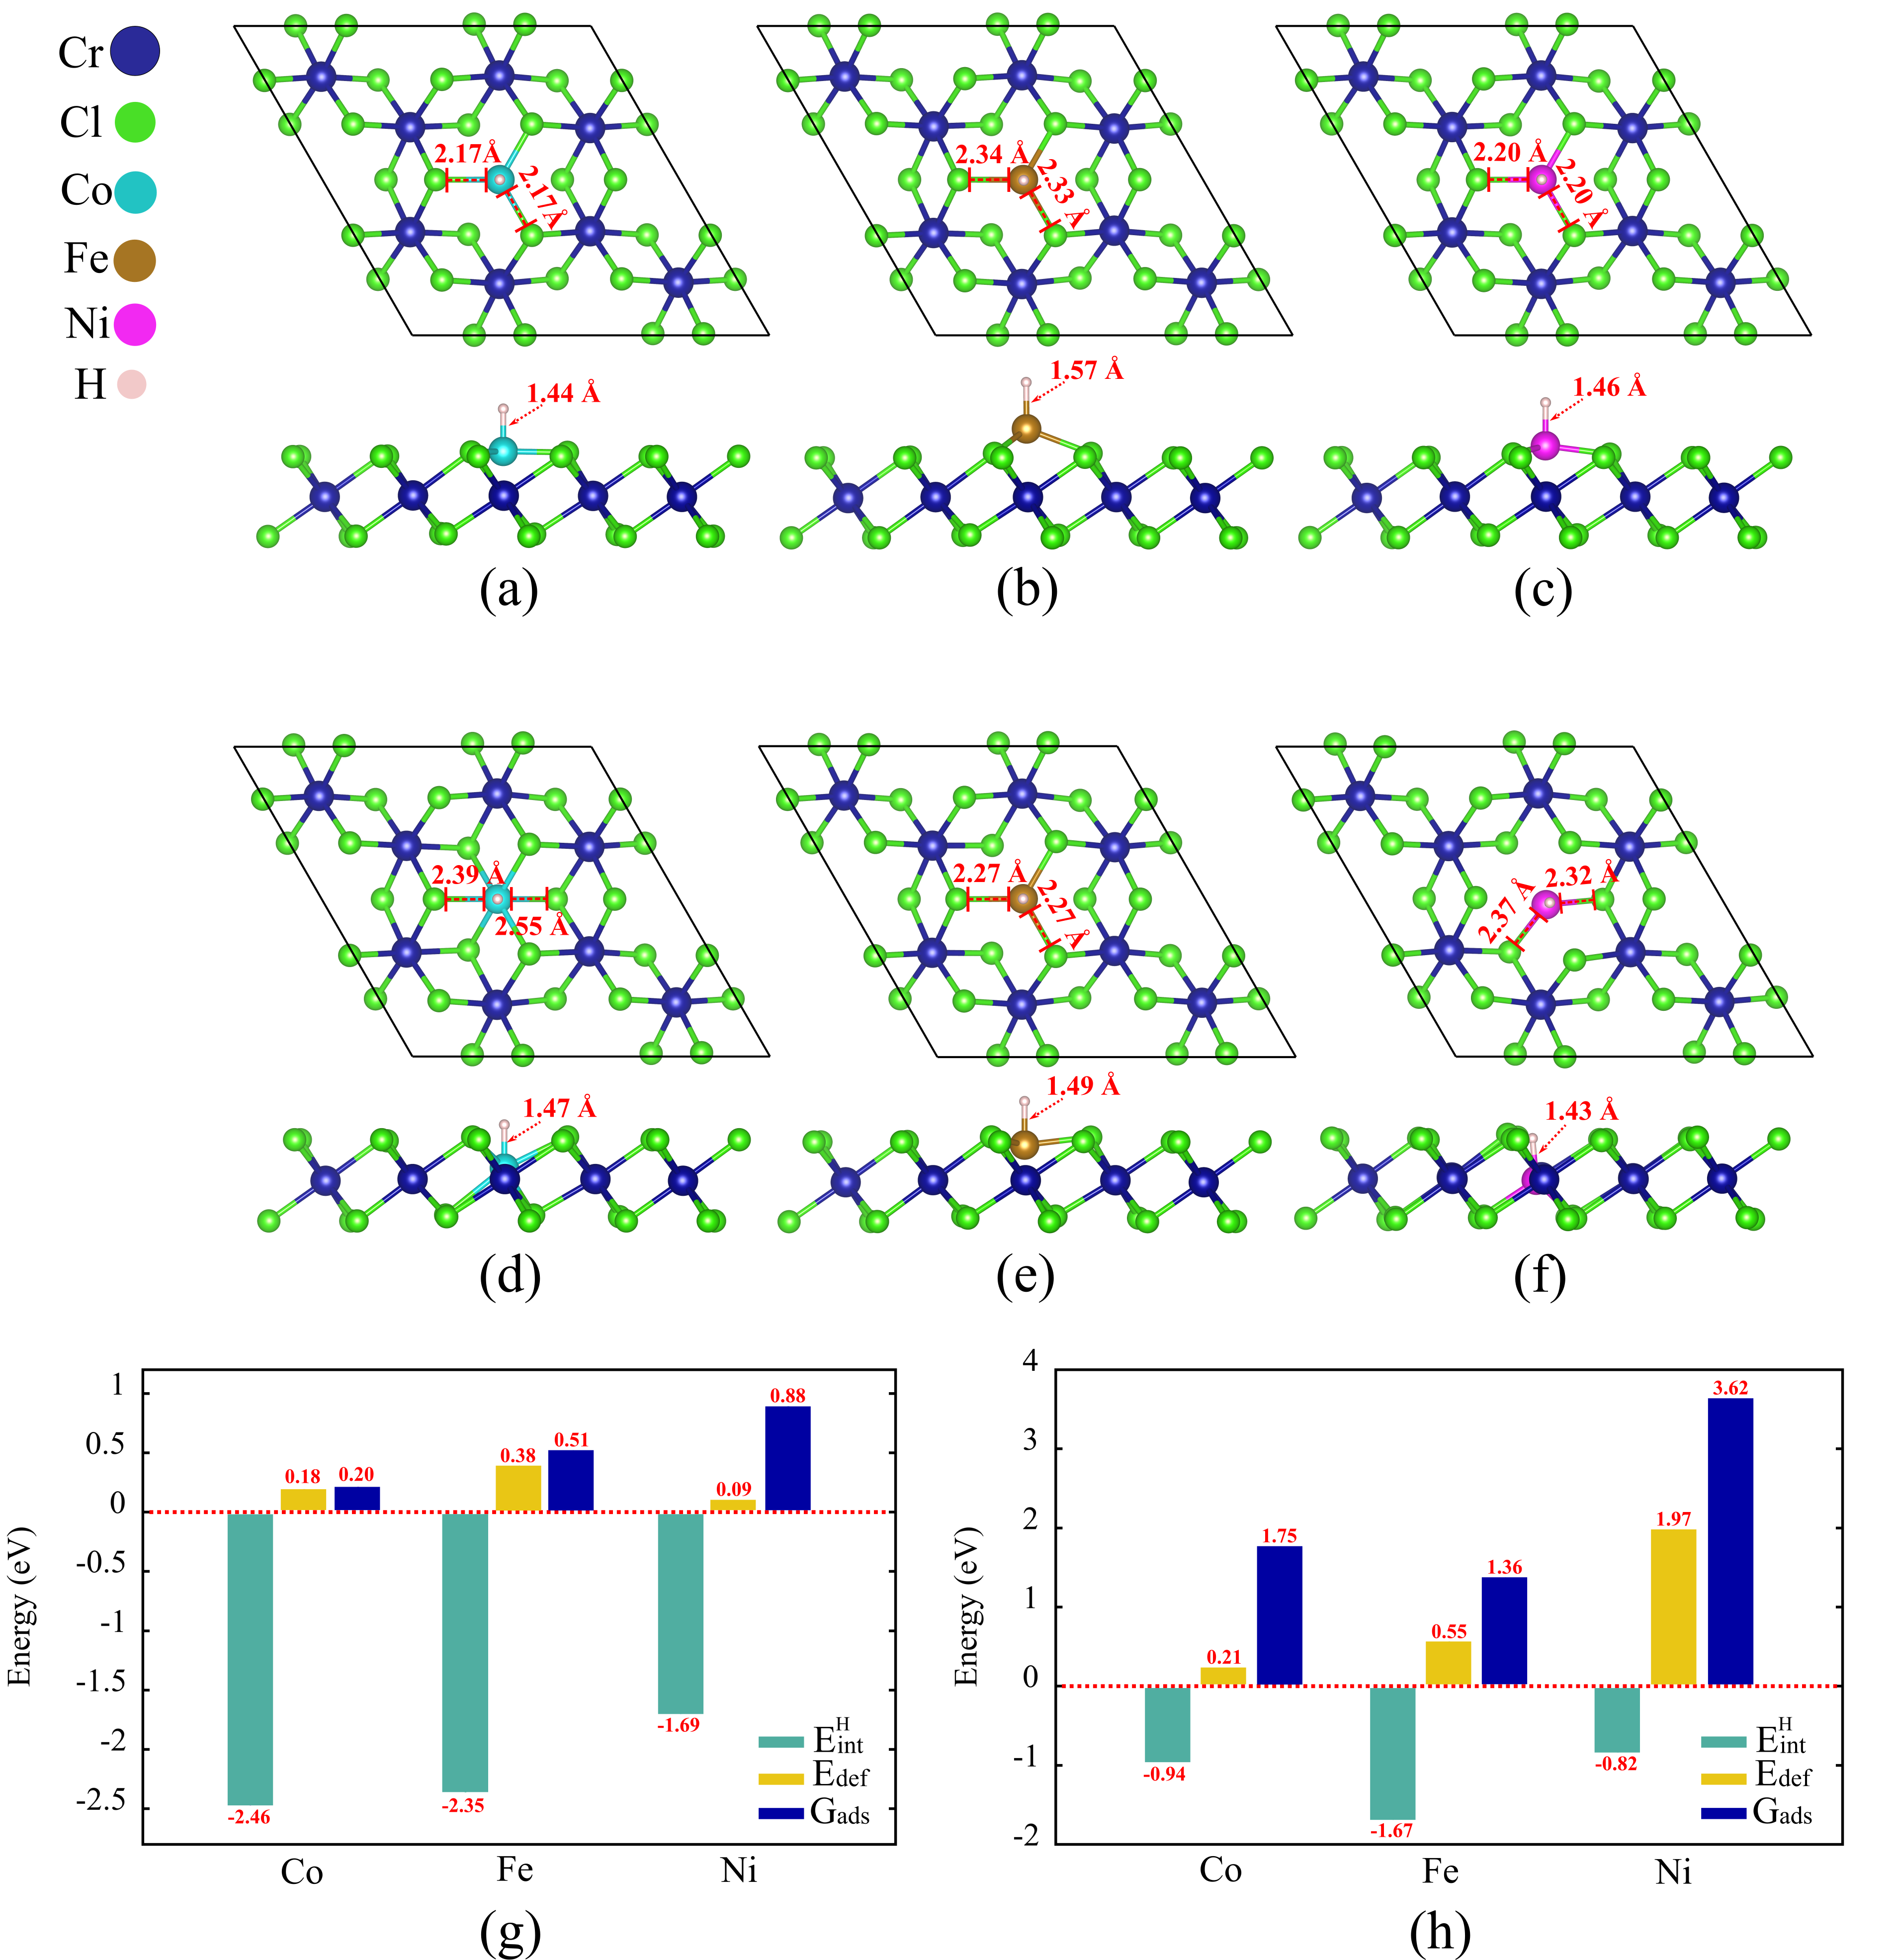
\includegraphics[width=1.0\textwidth]{figure/Fig7.png}
  \caption{Optimized H-adsorption geometries and energetic decomposition for transition-metal-functionalized monolayer CrCl$_3$. (a--c) Surface-adsorbed Co, Fe, and Ni after H adsorption. (d--f) Corresponding embedded configurations. Selected TM--H and local interatomic distances are indicated. (g,h) Atomic-H-referenced interaction energy, $E_{\mathrm{int}}^{\mathrm H}$, deformation energy, $E_{\mathrm{def}}$, and H adsorption free energy, $\Delta G_{\mathrm{ads}}$, for the surface-adsorbed and embedded structures.}
  \label{fig:Fig7}
\end{figure}

The reference states of the energetic quantities remain distinct. $E_{\mathrm{int}}^{\mathrm H}+E_{\mathrm{def}}$ yields the atomic-H-referenced adsorption energy, whereas $\Delta G_{\mathrm{ads}}$ is referenced to $\tfrac{1}{2}\mathrm{H}_2$ and includes the zero-point-energy and entropic correction. Because the same H/$\mathrm{H}_2$ reference offset applies to all configurations, the decomposition preserves the relative ordering and identifies whether an unfavorable $\Delta G_{\mathrm{ads}}$ originates primarily from weak H--surface interaction, structural deformation, or both.

The central trend is therefore controlled by coordination. Surface-exposed metals retain sufficient orbital and geometrical accessibility to bind H, whereas embedding increases TM--Cl coordination at the expense of H stabilization. Surface-adsorbed Co achieves the best compromise, with strong H interaction, limited deformation, and $\Delta G_{\mathrm{ads}}=0.20$~eV. Within the configurations and coverage examined here, it is the most favorable motif for H adsorption, although the calculated free energy alone does not establish the kinetics of the full HER pathway.

Within the computational hydrogen electrode framework, the theoretical HER overpotential is directly related to the adsorption free energy as $\eta = |\Delta G_{\mathrm{ads}}|/e$ for a single adsorption-limited step~\cite{Norskov_2005,Moraes2026,ASS2026_166886}. The calculated overpotentials are 0.20, 0.51, and 0.88~V for surface-adsorbed Co, Fe, and Ni, respectively, and range from 1.5 to 3.6~V for the embedded series. Surface-adsorbed Co therefore yields the lowest overpotential. Furthermore, within the Butler--Volmer framework for proton-coupled electron transfer, the exchange current density $i_0$ is maximized when $\Delta G_{\mathrm{ads}} \approx 0$~eV and decays symmetrically for both endergonic and exergonic adsorption~\cite{Norskov_2005}. The value $\Delta G_{\mathrm{ads}} = 0.20$~eV for surface-adsorbed Co places it closest to the peak of the exchange current density volcano among all configurations examined, further supporting its identification as the most catalytically favorable site.

The coordination dependence identified here is broadly consistent with previous studies showing that magnetic ordering and local electronic reconstruction can activate water-splitting sites in single-atom and atomically thin catalysts \cite{Sun2023,Duan2021}. Although those systems are chemically distinct from TM-functionalized CrCl$_3$, they support the general picture that spin polarization and coordination can jointly modify the electronic environment of hydrogen-binding centers. The present results further show that neither contribution should be considered independently of the structural response of the active site.

Figure~\ref{fig:Fig8} tests whether the occupied TM $d$-band center, $\varepsilon_d^{\mathrm{occ}}$, can rationalize the adsorption sequence using the electronic structure of the relaxed H-free systems. For the surface configurations, $\varepsilon_d^{\mathrm{occ}}$ shifts toward the Fermi level from Fe to Co and Ni, but $\Delta G_{\mathrm{ads}}$ follows the nonmonotonic order Co $<$ Fe $<$ Ni. Ni consequently has the occupied $d$-band center closest to $E_{\mathrm F}$ but the least favorable H adsorption within the surface family. The embedded systems are likewise nonmonotonic: Fe has the deepest occupied $d$-band center and the lowest $\Delta G_{\mathrm{ads}}$ of the embedded series, while Ni exhibits an intermediate $\varepsilon_d^{\mathrm{occ}}$ and the largest adsorption penalty.

The limited descriptor performance is consistent with the complexity of the spin-polarized TM-$3d$ manifolds. A spin-summed first moment does not retain the separate spin channels, orbital symmetry, crystal-field splitting, occupation of bonding and antibonding states, or the structural response induced by H adsorption. Moreover, each fitted family contains only three metals; the corresponding linear fits and $R^2$ values should therefore be interpreted as visual summaries rather than statistically predictive relationships. For the six configurations considered here, $\varepsilon_d^{\mathrm{occ}}$ is a complementary electronic indicator, not an independent predictor of $\Delta G_{\mathrm{ads}}$.

\begin{figure}[H]
  \centering
  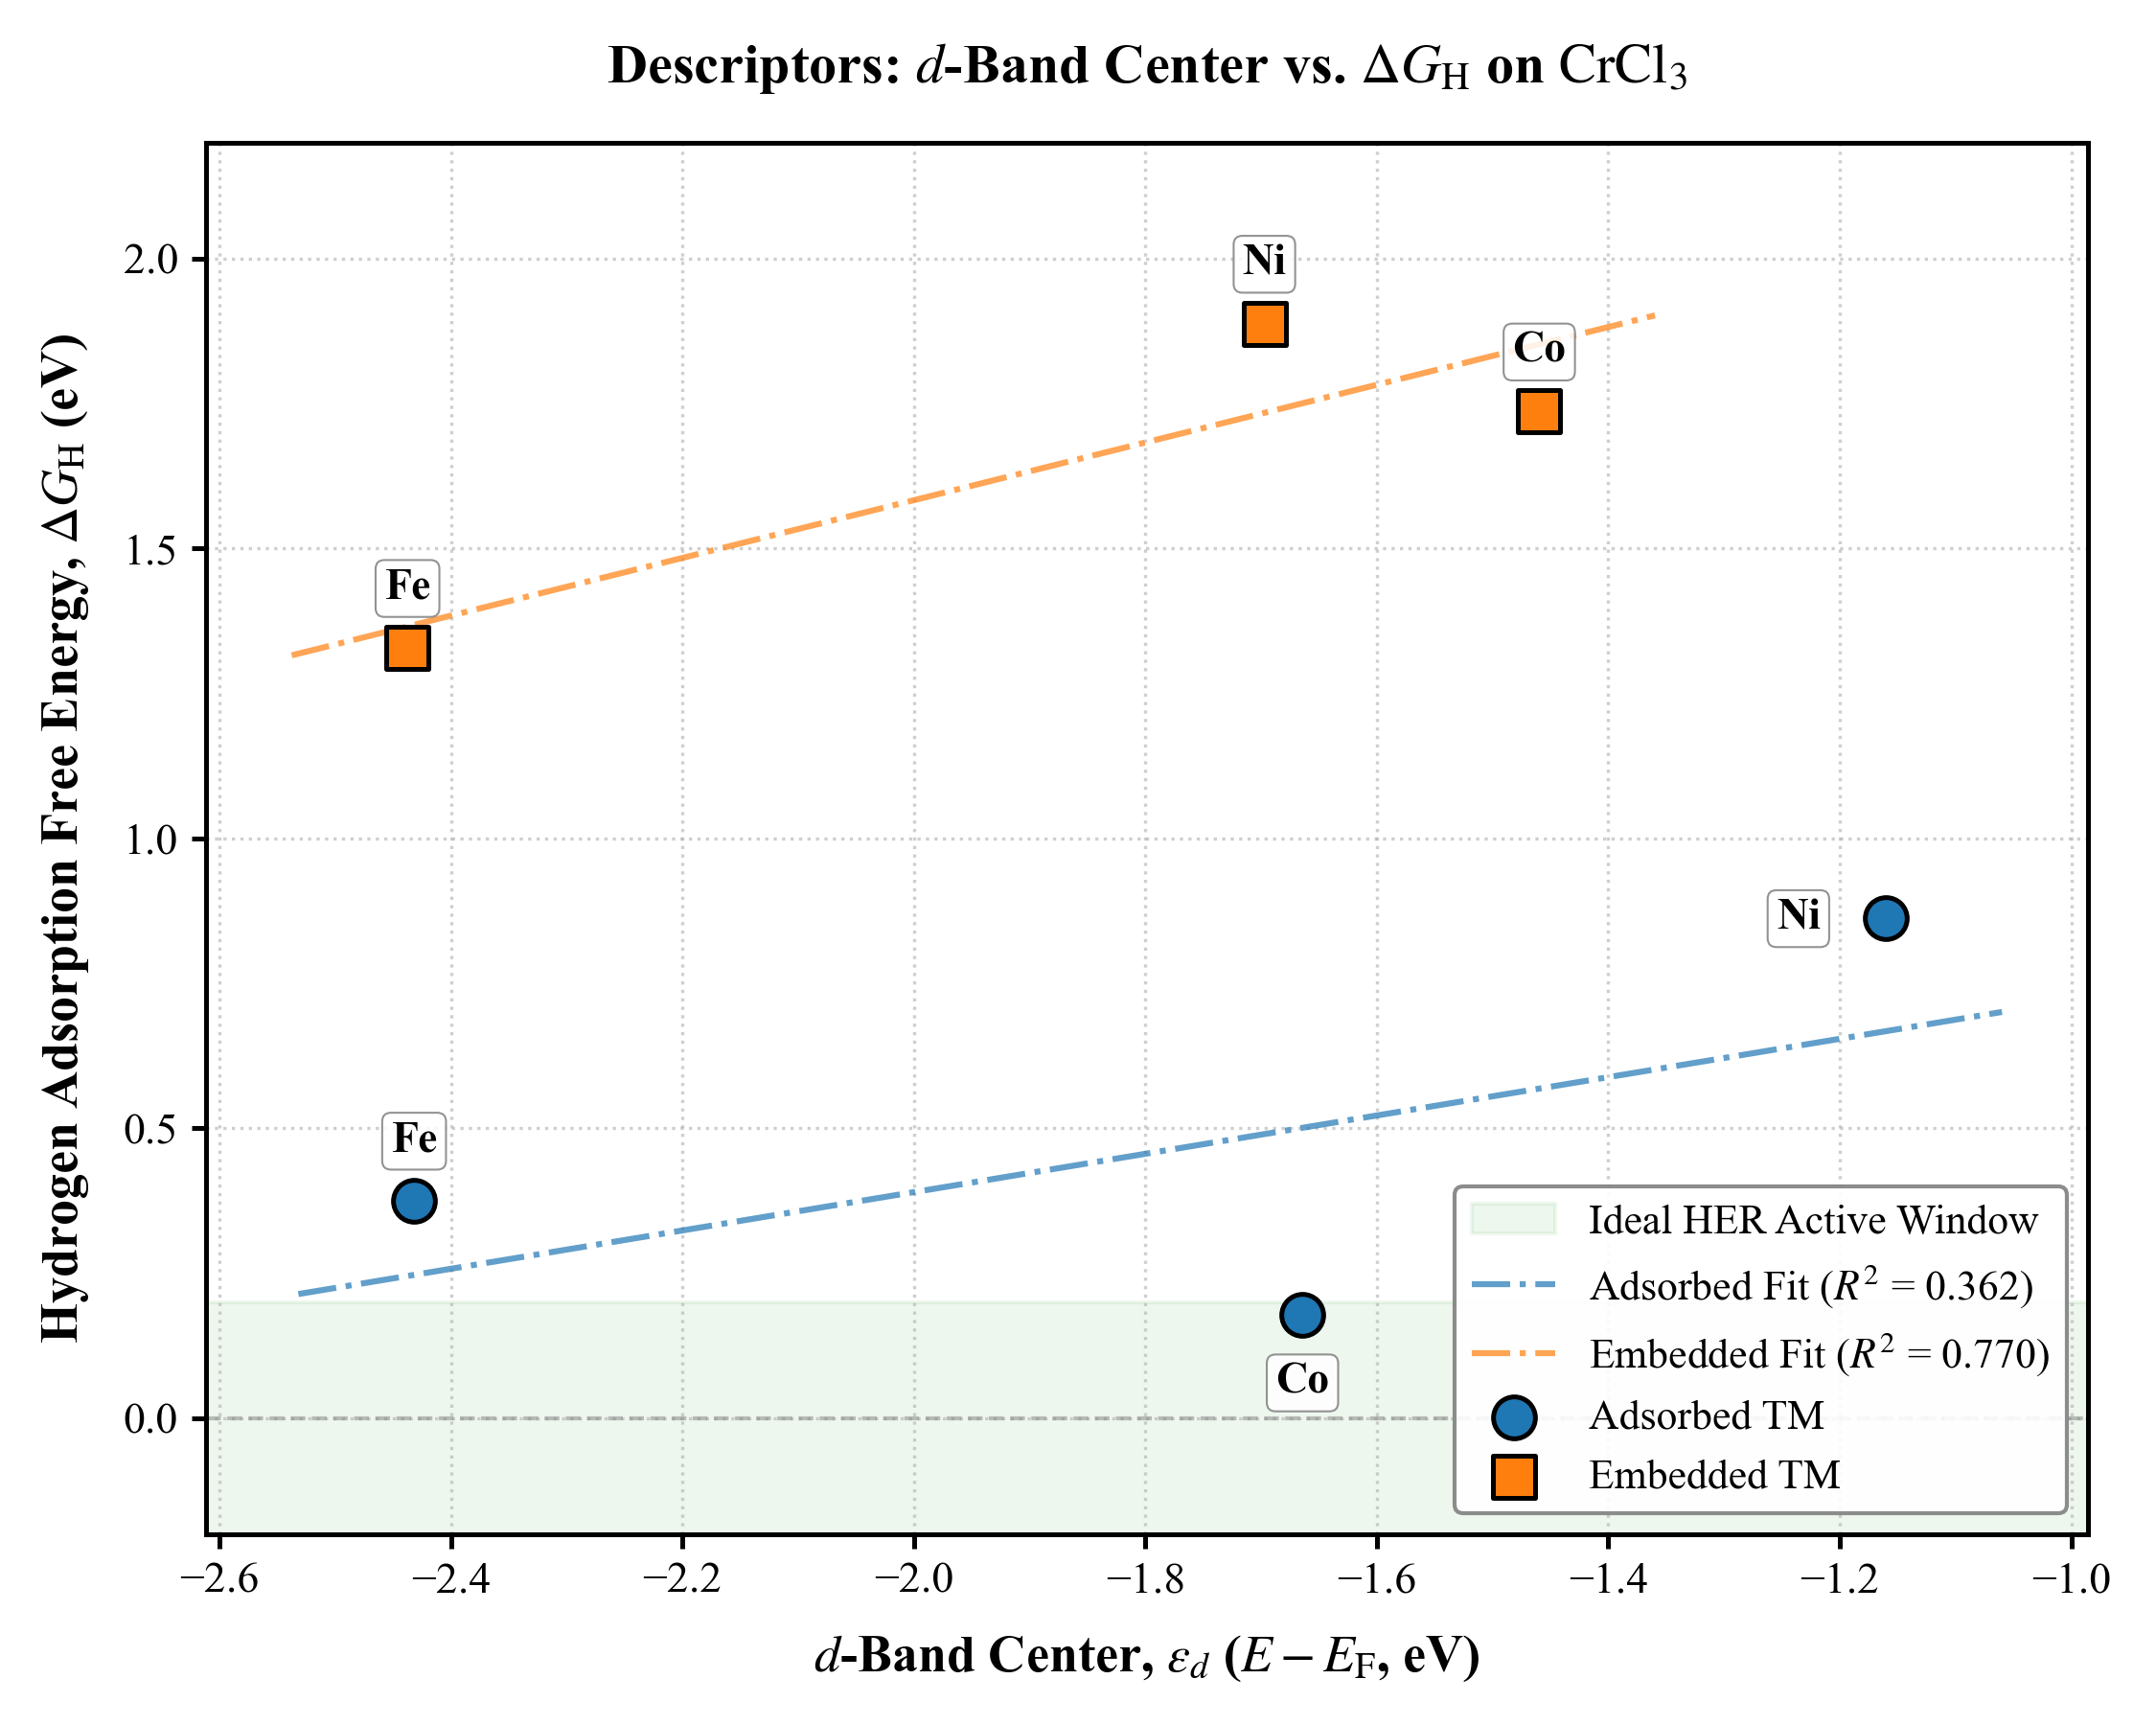
\includegraphics[width=1.0\linewidth]{figure/Fig8.png}
  \caption{Occupied $d$-band center, $\varepsilon_d^{\mathrm{occ}}$, versus H adsorption free energy, $\Delta G_{\mathrm{ads}}$, for surface-adsorbed and embedded Co, Fe, and Ni centers in monolayer CrCl$_3$. The linear fits are included only as visual guides because each coordination family contains three data points. The shaded region denotes $-0.2\leq\Delta G_{\mathrm{ads}}\leq0.2$~eV.}
  \label{fig:Fig8}
\end{figure}

This limitation should also be considered in the context of spin-dependent chemisorption. Cao and N{\o}rskov showed that exchange splitting produces nonlinear and adsorbate-dependent deviations from a simple $d$-band-center description on magnetic Fe, Co, and Ni surfaces \cite{doi:10.1021/acscatal.2c06319}. In their analysis, the minority-spin up-shift does not necessarily compensate for the weaker bonding associated with the downward displacement of the majority-spin states. They also found that the spin-induced variation in H adsorption is comparatively small relative to more spin-sensitive intermediates such as N. Although their work concerns extended metallic surfaces rather than atomically dispersed centers on CrCl$_3$, it supports the conclusion that a spin-summed first moment cannot, by itself, describe the adsorption response of a spin-polarized active site.

The local magnetic moment leads to the same conclusion (Figure~S5). Co provides the most favorable surface adsorption despite having neither the largest TM moment nor antiparallel polarization, and embedding changes the Ni moment only moderately while increasing its $\Delta G_{\mathrm{ads}}$ from 0.88 to 3.62~eV. Neither the magnitude nor the sign of the H-free local moment alone explains the adsorption trend.

Taken together, the structural, electronic, and energetic analyses show that H adsorption on TM-functionalized CrCl$_3$ is intrinsically multidimensional. The decisive factors are the coordination and exposure of the metal center, the distribution of TM--Cl bonding, the electronic structure available for TM--H interaction, and the deformation required to accommodate H. Surface-adsorbed Co provides the most favorable balance among these contributions, whereas the stronger integration of the embedded centers into the Cr--Cl framework systematically suppresses their H-binding thermodynamics.

\section{Conclusions}

Spin-polarized first-principles calculations demonstrate that transition-metal functionalization selectively modifies the hydrogen-adsorption thermodynamics of monolayer CrCl$_3$. The pristine Cl-terminated basal plane is unfavorable for H$^*$ formation, with the only locally retained adsorption configuration exhibiting $\Delta G_{\mathrm{ads}}=1.82$~eV. Surface-adsorbed Co, Fe, and Ni introduce exposed, spin-polarized $3d$ centers and reduce this thermodynamic penalty, with Co providing the most favorable value, $\Delta G_{\mathrm{ads}}=0.20$~eV. Notably, Ni interacts most strongly with the CrCl$_3$ substrate and shows a finite-temperature tendency toward deeper incorporation, but does not yield the strongest H binding. The combined structural, electronic, COHP, and energetic analyses reveal a coordination-controlled trade-off: increasing TM--Cl coordination enhances the integration of the metal center into the host lattice, while reducing its geometrical and orbital availability for interaction with H. Consequently, the embedded configurations exhibit substantially less favorable adsorption thermodynamics, particularly embedded Ni, for which weak H--surface interaction is accompanied by a large deformation penalty. Neither the occupied $d$-band center nor the local magnetic moment alone rationalizes the adsorption sequence, indicating that H binding is governed by the combined effects of local coordination, site exposure, electronic structure, and structural relaxation. These results identify surface-adsorbed Co as the most favorable H-binding motif among the configurations examined and establish coordination engineering as a promising strategy for tuning the reactivity of magnetic two-dimensional materials. The present analysis is restricted to thermodynamic descriptors within the computational hydrogen electrode framework, in which $\Delta G_{\mathrm{ads}}$ serves as the primary volcano-plot descriptor for the rate-limiting Volmer step. Full kinetic characterization via transition-state calculations (Volmer and Tafel barriers) and coverage-dependent free energy profiles represent critical directions for future work. Additionally, the calculations are performed for an ideal neutral monolayer in vacuum; solvation, applied potential, electrolyte effects, and surface reconstruction under realistic electrochemical conditions may shift the absolute $\Delta G_{\mathrm{ads}}$ values, and their inclusion via implicit-solvent or constant-potential DFT methods is identified as a further extension. Extension of the coordination engineering approach to the heavier CrX$_3$ homologs (X~=~Br, I) and to TM-functionalized MXenes, transition-metal dichalcogenides, and carbon-based supports would further establish the generality of the coordination-controlled trade-off identified here.

\section*{CRediT authorship contribution statement}
\begin{sloppypar}
  \textbf{Juan Rafael Gomez Quispe}: Conceptualization, Methodology, Software, Investigation, Writing - original draft. \textbf{Carlos Raul Primo Sapillado}: Investigation, Software, Validation. \textbf{Caique C. Oliveira}: Investigation, Software, Writing - review. \textbf{Chachi Rojas-Ayala}: Validation, Writing - review \& editing. \textbf{Pedro Alves da Silva Autreto}: Supervision, Project administration, Funding acquisition, Writing - review \& editing.
\end{sloppypar}

\section*{Declaration of competing interest}
The authors declare that they have no known competing financial interests or personal relationships that could have appeared to influence the work reported in this paper.

\section*{Acknowledgments}

C. C. O. acknowledges the S\~ao Paulo Research Foundation (FAPESP, process no. 2024/11376-6). P. A. S. A. acknowledges the Coordena\c{c}\~ao de Aperfei\c{c}oamento de Pessoal de N\'ivel Superior (CAPES, Finance Code 001), CNPq (grant no. 307390/2026-8), and the National Institute of Science and Technology on Materials Informatics (grant no. 371610/2023-0). This research was also supported by the Universidad Nacional Mayor de San Marcos under RR N$^\circ$ 011632-2024-R/UNMSM, through projects B2413006m and B2410003m. C. R. A. acknowledges PROCIENCIA--E041-2025-01 (contract no. PE501094353-2025). C. C. O., J. G. Q., and P. A. S. A. acknowledge the UFABC Computation Multiuser Center (CCM) for the computational resources provided. C. R. P. S., J. G. Q., and C. R. A. also acknowledge the LMSC-GMCAN laboratory for providing computational resources.

\section*{Data availability}

The optimized atomic structures (POSCAR files) for all seven configurations (pristine monolayer CrCl$_3$, and surface-adsorbed and embedded Co, Fe, and Ni) are provided in the Supporting Information. OUTCAR energy and magnetic-moment summaries, LOBSTER COHPCAR files, and AIMD XDATCAR trajectories will be deposited in a public repository upon acceptance; the DOI will be provided in the final published version. Additional data are available from the corresponding author upon reasonable request.

\bibliography{references}

\end{document}